\documentclass[lang=cn,newtx,10pt,scheme=chinese,usesamecnt]{elegantbook}

\title{线性代数习题课讲义}

\author{???}
\institute{KFRC}
\date{99999.13.32}
\version{1.0}


\setcounter{tocdepth}{3}

\logo{logo.jpg}
\cover{cover.png}

% 本文档命令
\usepackage{array}
\newcommand{\ccr}[1]{\makecell{{\color{#1}\rule{1cm}{1cm}}}}
\linespread{1.4}

% 修改标题页的橙色带
\definecolor{customcolor}{HTML}{1F1E33}
\colorlet{coverlinecolor}{customcolor}


\usepackage{cprotect}
\usepackage{xcolor}
\usepackage{biblatex}
\usepackage{listings}
\usepackage{graphicx}
\usepackage{amsmath}
\usepackage{mathdots}
\usepackage{extarrows}
\usepackage{tikz}
\usepackage{rotating}



\allowdisplaybreaks[4]


\elegantnewtheorem{homework}{作业}{prostyle}{exfancy}


\addbibresource[location=local]{reference.bib} % 参考文献,不要删除

\begin{document}

\maketitle
\frontmatter

\tableofcontents

\mainmatter

\chapter{矩阵之前}

    \section{作业解答}

    \subsection{周二}

        \begin{homework}[P114 T514]
            计算$\begin{bmatrix} 1 & 2 \\ 3 & 4 \end{bmatrix}^{100}$。
        \end{homework}

    \section{One More Thing}

        \subsection{数与数域}

            \subsubsection{复数与单位根}

                \begin{theorem}[Euler]
                    对于任意实数$\theta$,有$e^{i\theta}=\cos\theta+i\sin\theta$。特别地,当$\theta=\pi$时,有$e^{i\pi}+1=0$.
                \end{theorem}

                \begin{example}
                    计算$\sum\limits_{j=0}^n\cos j\theta$和$\sum\limits_{j=1}^n\sin j\theta$.
                \end{example}

                \begin{solution}
                    对$\theta =2k\pi$,有$\cos^{i}\theta = 1$,$\sin^{i}\theta = 0$,故$\sum\limits_{i=0}^n\cos i\theta = n+1$,$\sum\limits_{i=1}^n\sin i\theta = 0$.

                    对$\theta \neq 2k\pi$,令$T=\sum\limits_{j=1}^{n}e^{ij\theta}=\sum\limits_{j=0}^n\cos j\theta+i\sum\limits_{j=1} n\sin^{j}\theta$,有$e^{i\theta}T=T+e^{i(n+1)\theta}-1$,故$T=\dfrac{1-e^{i(n+1)\theta}}{1-e^{i\theta}}$.

                    分别计算实部虚部,有$\sum\limits_{i=0}^n\cos i\theta = \dfrac{1-\cos(n+1)\theta}{2(1-\cos\theta)}$,$\sum\limits_{i=1}^n\sin i\theta = \dfrac{\sin (n+1)\theta-\sin \theta}{2(1-\cos\theta)}$.
                \end{solution}

                \begin{definition}
                    $n$次单位根是指
                    \begin{equation}
                        \label{eq:unit_root}
                        \cos\frac{2k\pi}n+i\sin\frac{2k\pi}n, k=0,1,\cdots,n-1
                        \nonumber
                    \end{equation}
                    这n个复数,记$\omega_n=\cos\dfrac{2\pi}n+isin\dfrac{2\pi}n$,则他们可以写为$\omega_n^{0},\omega_n^{1},\cdots,\omega_n^{n-1}$。
                \end{definition}

                之所以叫单位根,是因为其满足

                \begin{proposition}[单位根的性质]
                    $n$次单位根是方程$x^n=1$的全部根.
                \end{proposition}

                根据\textbf{因式定理},可以推出

                \begin{equation}
                    \label{eq:unit_root_factor}
                    x^n-1=\prod_{k=0}^{n-1}(x-\omega_n^{k})
                    \nonumber
                \end{equation}

                对比各项系数可以得到一些恒等式。事实上最常用的为:

                \begin{proposition}[单位根恒等式]
                    \begin{enumerate}
                        \item
                            \begin{equation}
                                \label{eq:unit_root_identity1}
                                \sum_{k=0}^{n-1}(\omega_n^{k})^{m}=
                                \begin{cases}
                                    n & n \mid m \\
                                    0 & n \nmid m
                                \end{cases}
                                \nonumber
                            \end{equation}
                        \item
                            \begin{equation}
                                \label{eq:unit_root_identity2}
                                \omega_n^{a}=\omega_n^{a\pm n}
                                \nonumber
                            \end{equation}
                        \item
                            \begin{equation}
                                \label{eq:unit_root_identity3}
                                \overline{\omega_n^{a}}=\omega_n^{-a}
                                \nonumber
                            \end{equation}
                        \item
                            \begin{equation}
                                \label{eq:unit_root_identity4}
                                \omega_{mn}^{ma}=\omega_n^{a}
                                \nonumber
                            \end{equation}
                    \end{enumerate}
                \end{proposition}

                第二个恒等式就是最重要的\textbf{循环}性质。出于循环,它可以将一些东西按照模$n$的余数分类。

                \begin{example}
                    计算$\sum\limits_{k=0}^{\lfloor \frac{n}{3} \rfloor}\dbinom{n}{3k}$,$\dbinom{n}{m}$为组合数$C_n^{m}$,$\lfloor x\rfloor$为向下取整,即不大于$x$的最大整数。
                \end{example}

                \begin{solution}
                    考虑三次单位根$\omega_{3}=-\dfrac12+\dfrac{\sqrt{3}}{2}i$,由二项式定理有
                    \begin{equation}
                        \label{eq:binomial_step1}
                        (1+1)^n=\sum_{k=0}^n\binom{n}{k}=\binom{n}{0}+\binom{n}{1}+\binom{n}{2}+\binom{n}{3}+\binom{n}{4}+\cdots
                    \end{equation}
                    \begin{equation}
                        \label{eq:binomial_step2}
                        (1+\omega_{3})^n=\sum_{k=0}^n\binom{n}{k}\omega_{3}^{k}=\binom{n}{0}+\binom{n}{1}\omega_{3}+\binom{n}{2}\omega_{3}^{2}+\binom{n}{3}+\binom{n}{4}+\cdots
                    \end{equation}
                    \begin{equation}
                        \label{eq:binomial_step3}
                        (1+\omega_{3}^{2})^n=\sum_{k=0}^n\binom{n}{k}\omega_{3}^{2k}= \binom{n}{0}+\binom{n}{1}\omega_{3}^{2}+\binom{n}{2}\omega_{3}+\binom{n}{3}+\binom{n}{4}\omega_{3}^{2}+\cdots
                    \end{equation}
                    将(\ref{eq:binomial_step1}),(\ref{eq:binomial_step2})和(\ref{eq:binomial_step3})相加,注意到$1+\omega_{3}+\omega_{3}^{2}=0$,有
                    \begin{equation}
                        \label{eq:binomial_step4}
                        (1+1)^n+(1+\omega_{3})^n+(1+\omega_{3}^{2})^n=3\sum_{k=0}^{\lfloor \frac{n}{3} \rfloor}\binom{n}{3k}
                        \nonumber
                    \end{equation}
                    即有
                    \begin{equation}
                        \label{eq:binomial_step5}
                        \sum_{k=0}^{\lfloor \frac{n}{3} \rfloor}\binom{n}{3k}=\frac13(2^n+(1+\omega_{3})^n+(1+\omega_{3}^{2})^n)
                        \nonumber
                    \end{equation}
                \end{solution}

                \begin{exercise}
                    计算$\sum\limits_{k=0}^{\lfloor \frac{n-1}{3} \rfloor}\dbinom{n}{3k+1}$。
                \end{exercise}

                \begin{example}
                    \label{example:binomial}
                    计算$\sum\limits_{k=m}^n\dbinom{k}{m}$。
                \end{example}

                \begin{solution}
                    \begin{equation}
                        \label{eq:binomial_step6}
                        \binom{k}{m}=const\left(\frac{(1+x)^k}{x^m}\right),\text{其中}const(f(x))\text{表示}f(x)\text{的常数项}
                        \nonumber
                    \end{equation}
                    \begin{equation}
                        \label{eq:binomial_step7}
                        \Rightarrow \sum_{k=m}^n\binom{k}{m}=const\left(\sum_{k=m}^n\frac{(1+x)^k}{x^m}\right)=const\left(\frac1{x^{m}}\frac{(1+x)^{n+1}-(1+x)^{m}}{x}\right)=const\left(\frac{(1+x)^{n+1}}{x^{m+1}}\right)=\binom{n+1}{m+1}.
                        \nonumber
                    \end{equation}
                \end{solution}

                \begin{example}
                    单位圆内接正n边形$A_{1}A_{2}A_{3}\dots A_n$中,$P$为单位圆上一点,证明:$\sum\limits_{k=1}^n|PA_{k}|^{2}=2n$。
                \end{example}

                \begin{proof}

                    \begin{center}
                        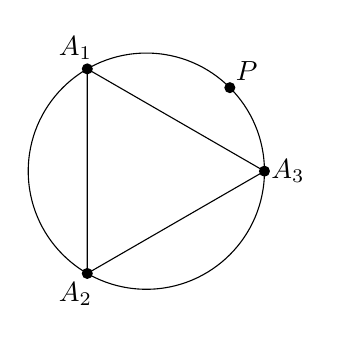
\begin{tikzpicture}
                            \draw (0,0) circle (1.5cm);
                            \coordinate (A1) at (120:1.5);
                            \coordinate (A2) at (240:1.5);
                            \coordinate (A3) at (0:1.5);
                            \coordinate (P) at (45:1.5);
                            \draw (A1) -- (A2) -- (A3) -- cycle;
                            \foreach \point in {A1, A2, A3, P}
                            \fill [black] (\point) circle (2pt);
                            \node at (120:1.8) {$A_1$};
                            \node at (240:1.8) {$A_2$};
                            \node at (0:1.8) {$A_3$};
                            \node at (45:1.8) {$P$};
                        \end{tikzpicture}
                    \end{center}

                    放在复平面上,设$A_{1}=\omega_n$,则$A_{k}=\omega_n^{k},\forall k=1,2,\cdots,n$。设$P=z$。

                    \begin{equation}
                        \label{eq:unit_circle_proof1}
                        \Rightarrow\sum_{k=1}^n|PA_{k}|^{2}=\sum_{k=1}^n|z-\omega_n^{k}|^{2}=\sum_{k=1}^n(z-\omega_n^{k})(\overline{z}-\overline{\omega_n^{k}})=\sum_{k=1}^n\left( 1-\omega_n^{k}\overline{z}-z\overline{\omega_n^{k}}+1 \right)=2n
                        \nonumber
                    \end{equation}

                    最后一个等号用到$\sum\limits_{k=1}^n\omega_n^{k}=0$。
                \end{proof}

            \subsubsection{数环、数域}

                \begin{definition}[数环、数域]
                    若复数域$\mathbb{C}$的某个包含1的子集$K$满足以下条件:
                    \begin{enumerate}
                        \item $a,b\in K\Rightarrow a+b\in K$;
                        \item $a,b\in K\Rightarrow a-b\in K$;
                        \item $a,b\in K\Rightarrow ab\in K$;
                    \end{enumerate}
                    则称$K$为数环。

                    若还满足$a\in K, a \neq 0\Rightarrow a^{-1}\in K$,则称$K$为数域。
                \end{definition}

                不难验证:

                \begin{proposition}[数环、数域-例子]
                    有理数集$\mathbb{Q}$、实数集$\mathbb{R}$、复数集$\mathbb{C}$都是数域。整数集$\mathbb{Z}$是数环但不是数域。
                \end{proposition}

                \begin{note}
                    当然,还有形态更复杂的数环和数域,例如所有$a+bi$在$a,b\in\mathbb{Z}$时构成数环,$a,b\in\mathbb{Q}$构成数域。
                \end{note}

                对于究竟怎样的集合是数环/数域,有一个简单的结论:

                \begin{proposition}[最小的数环、数域]
                    任何数环包含$\mathbb{Z}$,任何数域包含$\mathbb{Q}$。
                \end{proposition}

        \subsection{杂项}

            \subsubsection{求和符号练习}

            线性代数中求和符号是一个重要的工具,有时候可以用来简化问题,有时候可以用来构造问题。在中学时,我们知道$\sum\limits_{i=1}^{n}a_i=a_1+a_2+\cdots+a_n$,除此之外,还有多重求和及集合求和。以下给出定义:

            \begin{definition}[多重求和及集合求和]
                (1)(多重求和)$\sum\limits_{a_1,a_2,\cdots,a_m=1}^{n}x_{a_{1}a_{2}\cdots a_{m}}\triangleq \sum\limits_{a_1=1}^n\sum\limits_{a_2,a_3,\cdots,a_m=1}^{n}x_{a_{1}a_{2}\cdots a_{m}}=\cdots=\sum\limits_{a_1=1}^n\sum\limits_{a_2=1}^n\cdots\sum\limits_{a_m=1}^{n}x_{a_{1}a_{2}\cdots a_{m}}$

                (2)(集合求和)$\sum\limits_{e\in\Lambda}x_e$用于表示对集合$\Lambda$中所有元素$e$的$x_e$值求和。集合$\Lambda$是索引集合,可以是有限的或无限的。索引集合包含所有我们想要求和的索引$e$。对于集合$\Lambda$中的每个元素$e$,$x_e$表示与$e$相关联的数值。$\sum$表示对所有$x_e$进行累加,其中$e$遍历集合$\Lambda$的所有元素。例如$\sum\limits_{i=1}^{n}a_i=\sum\limits_{e\in \{1,2,\cdots,n\}}a_e$。

                集合$\Lambda$也可以被替换为某一条件,例如$\sum\limits_{i=1}^{n}a_i=\sum\limits_{1\leq i\leq n}a_i,\sum\limits_{1\leq i<j\leq n}a_{ij}=\sum\limits_{i=1}^n\sum\limits_{j=i+1}^{n}a_{ij}$
            \end{definition}

            下面是一些求和符号的练习。

            \begin{example}
                证明:$\sum\limits_{i=1}^n\sum\limits_{j=1}^{m}a_{i}{b_j}=\sum\limits_{j=1}^{m}\sum_{i=1}^{n}a_{i}{b_j}=\left(\sum\limits_{i=1}^{n}a_{i}\right) \left(\sum\limits_{j=1}^{m}b_{j}\right)$
            \end{example}

            \begin{proof}
                显然矩阵
                $\begin{bmatrix}
                    a_{1}b_{1} & a_{1}b_{2} & \cdots & a_{1}b_{m} \\
                    a_{2}b_{1} & a_{2}b_{2} & \cdots & a_{2}b_{m} \\
                    \vdots & \vdots & \ddots & \vdots \\
                    a_{n}b_{1} & a_{n}b_{2} & \cdots & a_{n}b_{m}
                \end{bmatrix}$
               的元素按行求和等于按列求和,故得证。
            \end{proof}

            \begin{example}
                计算$\sum\limits_{i=1}^n\sum\limits_{j=1}^n(i+j)^{2}$
            \end{example}

            \begin{solution}
                \begin{equation*}
                    \begin{split}
                        \sum\limits_{i=1}^n\sum\limits_{j=1}^n(i+j)^{2}&=\sum\limits_{i=1}^n\sum\limits_{j=1}^n(i^{2}+j^{2}+2ij)=n\sum\limits_{i=1}^{n}i^{2}+\sum\limits_{j=1}^{n}j^{2}+2\sum\limits_{i=1}^n\sum\limits_{j=1}^{n}ij=2n\cdot\dfrac{n(n+a)(2n+1)}6+2\left(\sum\limits_{i=1}^{n}i\right)\left(\sum\limits_{j=1}^{n}j\right) \\
                                                                           &=\dfrac{n^2(n+1)(2n+1)}3+2\left(\dfrac{n(n+1)}2\right)^{2}=\dfrac{n^2(n+1)(7n+5)}6
                    \end{split}
                \end{equation*}
            \end{solution}

            \begin{example}[(Chebyshev)]
                若$a_{1}\leq a_{2}\leq\cdots\leq a_n,b_{1}\leq b_{2}\leq\cdots\leq b_n$,则$\left(\sum\limits_{i=1}^{n}a_{i}\right)\left(\sum\limits_{j=1}^{n}b_{j}\right)\leq n\sum\limits_{k=1}^{n}a_{k}b_{k}$。
            \end{example}

            \begin{proof}
                只需证明$n\sum\limits_{k=1}^{n}a_{k}b_{k}-\left(\sum\limits_{i=1}^{n}a_{i}\right)\left(\sum\limits_{j=1}^{n}b_{j}\right)=\sum\limits_{1\leq j<i\leq n}(a_{i}-a{j})(b_{i}-b_{j})\geq 0$。令$S=\sum\limits_{1\leq j<i\leq n}(a_{i}-a{j})(b_{i}-b_{j})$.
                \begin{equation*}
                    \begin{split}
                        2S&=\sum_{1\leq j<i\leq n}(a_{i}-a_{j})(b_{i}-b_{j})+\sum_{1\leq i<j\leq n}(a_{j}-a_{i})(b_{j}-b_{i})=\sum_{i,j=1}^n(a_{j}-a_{i})(b_{j}-b_{i}) \\
                          &=\sum_{i,j=1}^n(a_{j}b_{j}+a_{i}b_{i}-a_{i}b_{j}-a_{j}b_{i})=2n\sum_{k=1}^{n}a_{k}b_{k}-2\sum_{i,j=1}^{n}a_{i}b_{j}=2\left(n\sum_{k=1}^{n}a_{k}b_{k}-\left(\sum\limits_{i=1}^{n}a_{i}\right)\left(\sum\limits_{j=1}^{n}b_{j}\right)\right)
                    \end{split}
                \end{equation*}
            \end{proof}

            \begin{example}
                记$H_{k}=\sum\limits_{j=1}^{k}\dfrac1j$,(1)求$\sum\limits_{1\leq j<k\leq n}\dfrac1{k-j}$(用$H_{k}$表示),(2)证明$\sum\limits_{j=1}^{n-1}H_{j}=nH_n-n$。
            \end{example}

            \begin{solution}
                $ $

                (1)$\sum\limits_{1\leq j<k\leq n}\dfrac1{k-j}=\sum\limits_{k=2}^n\sum\limits_{j=1}^{k-1}\dfrac1{k-j}=\sum\limits_{k=2}^n\sum\limits_{j=1}^{k-1}\dfrac1j=\sum\limits_{k=2}^{n}H_{k-1}=\sum\limits_{k=1}^{n-1}H_{k}$

                (2)$\sum\limits_{j=1}^{n-1}H_{j}=\sum\limits_{j=1}^{n-1}\sum\limits_{l=1}^{j}\dfrac1l=\sum\limits_{l=1}^{n-1}\sum\limits_{j=l}^{n-1}\dfrac1l=\sum\limits_{l=1}^{n-1}\dfrac{n-l}l=\sum\limits_{l=1}^n\dfrac{n-l}l=\sum\limits_{l=1}^n\left(\dfrac{n}l-1\right)=nH_n-n$
            \end{solution}

            \begin{example}[(Abel)]
                记$B_n=\sum\limits_{i=1}^{n}b_i$,则$S=\sum\limits_{i=1}^{n}a_{i}b_i=B_{n}a_n-\sum\limits_{i=1}^{n-1}B_i(a_{i+1}-a_i)$。
            \end{example}

            \begin{proof}
                \begin{equation*}
                    \begin{split}
                        \sum_{i=1}^{n}a_{i}b_i&=\sum_{i=1}^{n}a_{i}(B_i-B_{i-1})=\sum_{i=1}^{n}a_{i}B_{i}-\sum_{i=1}^{n}a_{i}B_{i-1}=a_{n}B_{n}+\sum_{i=1}^{n-1}a_{i}B_{i}-\sum_{i=0}^{n-1}a_{i+1}B_i \\
                                              &=a_{n}B_{n}+\sum_{i=1}^{n-1}(a_{i}-a_{i+1})B_i-a_{1}B_{0}=B_{n}a_n-\sum_{i=1}^{n-1}B_i(a_{i+1}-a_i)
                    \end{split}
                \end{equation*}
            \end{proof}

        \subsubsection{组合恒等式}

            \begin{lemma}
                \label{lemma:combinatorial_identity}
                \begin{enumerate}
                    \item
                        \begin{equation*}
                            \binom{n}{k}=\binom{n}{n-k}(0\leq k\leq n)
                        \end{equation*}
                    \item
                        \begin{equation*}
                            k\binom{n}{k}=n\binom{n-1}{k-1}
                        \end{equation*}
                    \item
                        \begin{equation*}
                            \binom{n}{m}+\binom{n}{m+1}=\binom{n+1}{m+1}
                        \end{equation*}
                \end{enumerate}
            \end{lemma}

            \begin{theorem}[二项式定理]
                对$\forall x\in \mathbb{R}$及$n\in \mathbb{N}^*$,有$(1+x)^n=\sum\limits_{k=0}^{n}\dbinom{n}{k}x^{k}$。
            \end{theorem}

            \begin{proof}
                归纳。利用引理\ref{lemma:combinatorial_identity}\textbf{(3)},有
                \begin{equation*}
                    (1+x)^n=(1+x)\cdot(1+x)^{n-1}=(1+x)\sum_{k=0}^{n-1}\binom{n-1}{k}x^{k}=\sum_{k=1}^{n-1}\left(\binom{n-1}{k-1}+\binom{n-1}{k}\right)x^{k}+1+x^n=\sum_{k=0}^{n}\binom{n}{k}x^{k}
                \end{equation*}
            \end{proof}

            \begin{corollary}
                利用上述定理和引理,可以得到:
                \begin{enumerate}
                    \item
                        \begin{equation*}
                            \sum_{k=0}^{n}\binom{n}{k}=2^{n}
                        \end{equation*}
                    \item
                        \begin{equation*}
                            \sum_{\substack{0\leq k\leq n \\ k\text{为偶数}}}\binom{n}{k}=\sum_{\substack{0\leq k\leq n \\ k\text{为奇数}}}\binom{n}{k}=2^{n-1}
                        \end{equation*}
                    \item
                        \begin{equation*}
                            \binom{m+n}{k}=\sum_{i=0}^{k}\binom{m}{i}\binom{n}{k-i}\text{。特别地,}\binom{2n}{n}=\sum_{i=0}^{n}\binom{n}{i}^{2}
                        \end{equation*}
                    \item
                        \begin{equation*}
                            \sum_{k=0}^{n}k\binom{n}{k}=n2^{n-1}
                        \end{equation*}
                    \item
                        \begin{equation*}
                            \sum_{k=m}^{n}\binom{k}{m}=\binom{n+1}{m+1}
                        \end{equation*}
                    \item
                        \begin{equation*}
                            \sum_{k=0}^{n}\binom{m+k}{k}=\binom{m+n+1}{n}
                        \end{equation*}
                \end{enumerate}
            \end{corollary}

            \begin{proof}
                (1)(2)对$(1+x)^n$使用二项式定理,分别取$x=1$和$x=-1$即可。

                (3)注意到$(1+x)^{m+n}=(1+x)^n\cdot(1+x)^m$,分别使用二项式定理,展开后比较$x^{k}$系数。

                (4)$(1+x)^n=\sum\limits_{k=0}^{n}\dbinom{n}{k}x^{k}$两侧对$x$求导,并取$x=1$即可。

                (5)见例题\ref{example:binomial}。

                (6)利用引理\ref{lemma:combinatorial_identity}\textbf{(3)}归纳即可。
            \end{proof}

            \begin{example}
                设$n\leq m$,证明:$\sum\limits_{k=0}^{m}\dbinom{m}{k}\dbinom{n+k}{m}=\sum\limits_{k=0}^{m}\dbinom{m}{k}\dbinom{n}{k}2^k$。
            \end{example}

            \begin{proof}
                \begin{equation*}
                    \begin{split}
                        \sum\limits_{k=0}^{m}\dbinom{m}{k}\dbinom{n+k}{m}&=[x^m](1+x)^n\sum_{k=0}^m\binom{m}{k}(1+x)^n=[x^m](1+x)^{n}(2+x)^m \\
                                                                         &=[x^m](1+x)^n\sum_{k=0}^m\binom{m}{k}2^{k}x^{m-k}=\sum_{k=0}^{m}\dbinom{m}{k}\dbinom{n}{k}2^k
                    \end{split}
                \end{equation*}
                其中$[x^m]f(x)$表示多项式$f(x)$的$m$次项系数。
            \end{proof}

\chapter{行列式}

    \section{作业解答}

    \section{更多、更多的行列式}

        \subsection{行列式的定义}

            行列式具有多种定义,以下只列出常见的三种,请读者自行验证它们的等价性。

            逆序数定义又称为行列式的完全展开定义。具体表述为:

            \begin{definition}[逆序数定义]
                \label{def_det:inverse_order}
                设$A=(a_{ij})_{n\times n}$是$n$阶方阵,定义行列式
                \begin{equation*}
                    \det A =\det
                    \begin{bmatrix}
                        a_{11} & a_{12} & \cdots & a_{1n} \\
                        a_{21} & a_{22} & \cdots & a_{2n} \\
                        \vdots & \vdots & \ddots & \vdots \\
                        a_{n1} & a_{n2} & \cdots & a_{nn}
                    \end{bmatrix}
                    \triangleq\sum_{\sigma\in S_n}2(\chi_{A_n}(\sigma))-\frac12)a_{1\sigma(1)}a_{2\sigma(2)}\cdots a_{n\sigma(n)}
                \end{equation*}
                其中$\chi$是示性函数,$S_n$是$n$阶置换群,$A_n$是$n$阶交错群。
            \end{definition}

            \begin{note}
                \,$2(\chi_{A_n}(\sigma))-\dfrac12)$本质上是检验置换$\sigma$的奇偶性。对$\sigma=\begin{pmatrix}1 & 2 & \cdots & n \\ j_1 & j_2 & \cdots & j_n \end{pmatrix}$,$2(\chi_{A_n}(\sigma))-\dfrac12)\equiv (-1)^{\tau(j_1,j_2,\cdots,j_n)}$。
            \end{note}

            $ $

            归纳法定义又称为按行展开法定义。该定义直接给出了行列式的计算式(展开式)。

            \begin{definition}[归纳法定义]
                \label{def_det:induction}
                设$A=(a_{ij})_{n\times n}$是$n$阶方阵,定义行列式$\det A$是按下列法则确定的一个数:
                \begin{enumerate}
                    \item 当$n=1$时,$\det a_{11}=a_{11}$;
                    \item 当$n\geq 2$时,$\det A=\sum\limits_{j=1}^{n}a_{1j}A_{1j}$,其中$A_{1j}$是$A$中元$a_{1j}$的代数余子式。
                \end{enumerate}
            \end{definition}

            由这一定义可以得到:

            \begin{theorem}[Laplace展开定理]
                \label{thm_det:Laplace}
                设A是$n$阶方阵,$A=(a_{ij})_{n\times n}$,对任意正整数$r<n$,任意取定$r$个指标$1\leq i_1<i_2,\cdots<i_r\leq n$,则$\det A$的值等于它的第$i_1,i_2,\cdots,i_r$行(或列)元组成的所有$r$阶子式分别与它们的代数余子式的乘积之和。即
                \begin{equation*}
                    \begin{split}
                        \det A &= \sum_{1\leq j_1<j_2<\cdots<j_r\leq n}A\begin{pmatrix} i_1 & i_2 & \cdots & i_r \\ j_1 & j_2 & \cdots & j_r\end{pmatrix}(-1)^{\sum\limits_{k=1}^{r}(i_k +j_k)}A\begin{pmatrix}i_{r+1} & i_{r+2} & \cdots & i_n \\ j_{r+1} & j_{r+2} & \cdots & j_n\end{pmatrix} \\
                               &= \sum_{1\leq j_1<j_2<\cdots<j_r\leq n}A\begin{pmatrix} j_1 & j_2 & \cdots & j_r \\ i_1 & i_2 & \cdots & i_r\end{pmatrix}(-1)^{\sum\limits_{k=1}^{r}(i_k +j_k)}A\begin{pmatrix}j_{r+1} & j_{r+2} & \cdots & j_n \\ i_{r+1} & i_{r+2} & \cdots & i_n\end{pmatrix}
                    \end{split}
                \end{equation*}
                其中$i_{r+1},i_{r+2},\cdots,i_n$是由$1,2,\cdots,n$去掉$i_1,i_2,\cdots,i_r$后剩下的数按从小到大排列得到,$j_{r+1},j_{r+2},\cdots,j_n$是由$1,2,\cdots,n$去掉$j_1,j_2,\cdots,j_r$后剩下的数按从小到大排列得到。
            \end{theorem}

            \begin{proof}
                此定理的证明已超出线性代数B1的范围,但是可以参考《线性代数(李炯生\quad 查建国\quad 王新茂)》教材的2.3节。
            \end{proof}

            \begin{example}
                设$\det A$是$n$阶行列式,正整数$r<n$。若$\det A$的所有$r$阶子式都等于零,证明:$\det A=0$。
            \end{example}

            \begin{proof}
                由Laplace展开定理,$\det A$的$r$阶子式等于零,有$\det A$的展开式中求和的每一项都是$0$,故$\det A=0$。
            \end{proof}

            行列式的公理化定义将行列式归结为满足3条性质的线性映射,而不是直接给出行列式的具体形式。

            $ $

            \begin{definition}[公理化定义]
                $n$维向量空间$\mathbb{F}^n$上的规范反对称$n$重线性函数称为数域$\mathbb{F}$上$n$阶行列式函数,简称$n$阶行列式。

                换言之,行列式函数$\det:\mathbb{F}^{n}\times\mathbb{F}^{n}\times\cdots\times\mathbb{F}^{n}\rightarrow\mathbb{F}$是满足以下三条性质的函数:
                \begin{enumerate}
                    \item 规范性:$\det(e_1,e_2,\cdots,e_n)=1$,其中$e_1,e_2,\cdots,e_n$是$\mathbb{F}^n$的一组标准正交基;
                    \item 反对称性:$\forall 1\leq i<j\leq n,\det(\cdots,\alpha_i,\cdots,\alpha_j,\cdots)=-\det(\cdots,\alpha_j,\cdots,\alpha_i,\cdots)$;
                    \item 线性性:$\forall \lambda,\mu\in\mathbb{F},\det(\lambda\alpha_1+\mu\beta_1,\alpha_2,\cdots,\alpha_n)=\lambda\det(\alpha_1,\alpha_2,\cdots,\alpha_n)+\mu\det(\beta_1,\alpha_2,\cdots,\alpha_n)$。
                \end{enumerate}
            \end{definition}

        \subsection{行列式计算练习}

            矩阵/行列式打洞的神秘技巧并不是线性代数的核心,但为了考试,请大家务必掌握。

            \subsubsection{定义法/降阶法/化为上三角}

                \begin{example}
                    计算$\det \begin{bmatrix}1&0&1&4\\-1&-3&-4&-2\\2&-1&4&4\\2&3&-3&2\end{bmatrix}$。
                \end{example}

                \begin{solution}
                    \begin{equation*}
                        \begin{split}
                            \det \begin{bmatrix}1&0&1&4\\-1&-3&-4&-2\\2&-1&4&4\\2&3&-3&2\end{bmatrix}&\xlongequal[-2r_1\rightarrow r_4]{\substack{r_1\rightarrow r_2\\-2r_1\rightarrow r_3}}\det \begin{bmatrix}1&0&1&4\\0&-3&-3&-6\\0&-1&2&12\\0&3&-5&10\end{bmatrix}\xlongequal{r_2\leftrightarrow r_3}\det \begin{bmatrix}1&0&1&4\\0&-1&2&12\\0&-3&-3&-6\\0&3&-5&10\end{bmatrix} \\
                                                                                                     &\xlongequal[3r_2\rightarrow r_4]{-3r_2\rightarrow r_3}\det \begin{bmatrix}1&0&1&4\\0&-1&2&12\\0&0&-9&-42\\0&0&1&46\end{bmatrix}=-1\cdot(-1)\cdot \det\begin{bmatrix}-9&-42\\1&46\end{bmatrix}=-372
                        \end{split}
                    \end{equation*}
                \end{solution}

                \begin{example}
                    计算$\det \begin{bmatrix}0&0&0&1&0\\0&0&3&2&0\\0&5&4&0&0\\9&8&7&6&0\\13&12&11&0&10\end{bmatrix}$。
                \end{example}

                \begin{solution}
                    \begin{equation*}
                        \begin{split}
                            \det \begin{bmatrix}0&0&0&1&0\\0&0&3&2&0\\0&5&4&0&0\\9&8&7&6&0\\13&12&11&0&10\end{bmatrix}&\xlongequal{\text{第一行展开}}(-1)^{1+4}\det\begin{bmatrix}0&0&3&0\\0&5&4&0\\9&8&7&0\\13&12&11&10\end{bmatrix}\xlongequal{\text{第一行展开}}-(-1)^{1+3}\cdot 3\det\begin{bmatrix}0&5&0\\9&8&0\\13&12&10\end{bmatrix} \\
                                                                                                                      &\xlongequal{\text{第一行展开}}-(-1)^{1+2}\cdot15\det\begin{bmatrix}9&0\\13&10\end{bmatrix}=15\cdot 90=1350
                        \end{split}
                    \end{equation*}
                \end{solution}

                \begin{example}
                    计算$\det \begin{bmatrix}x&y&&&\\&x&y&&\\&&x&\ddots&\\&&&\ddots&y\\y&&&&x\end{bmatrix}_{n\times n}$。
                \end{example}

                \begin{solution}
                    $\det \begin{bmatrix}x&y&&&\\&x&y&&\\&&x&\ddots&\\&&&\ddots&y\\y&&&&x\end{bmatrix}\xlongequal{\text{第一列展开}}x\cdot\det\begin{bmatrix}x&y&&\\&x&\ddots&\\&&\ddots&y\\&&&x\end{bmatrix}+(-1)^{n+1}y\cdot\begin{bmatrix}y&&&\\x&y&&\\&\ddots&\ddots&\\&&x&y\end{bmatrix}=x^n+(-1)^{n+1}y^n$
                \end{solution}

                \begin{note}
                    有一定规律(元素大量重复)矩阵化为上三角的重要结构:$(1,1,\cdots,1)$
                \end{note}

                \begin{example}
                    计算$\det\begin{bmatrix}1&1&1&1\\a&b&c&d\\a^2&b^2&c^2&d^2\\a^4&b^4&c^4&d^4\end{bmatrix}$
                \end{example}

                \begin{solution}
                    \begin{align*}
                             &\det\begin{bmatrix}1&1&1&1\\a&b&c&d\\a^2&b^2&c^2&d^2\\a^4&b^4&c^4&d^4\end{bmatrix}\xlongequal[-a^4 r_1\rightarrow r_4]{\substack{-ar_1\rightarrow r_2\\-a^2 r_1\rightarrow r_3}}\det\begin{bmatrix}1&1&1&1\\0&b-a&c-a&d-a\\0&b^2-a^2&c^2-a^2&d^2-a^2\\0&b^4-a^4&c^4-a^4&d^4-a^4\end{bmatrix}=\det\begin{bmatrix}b-a&c-a&d-a\\b^2-a^2&c^2-a^2&d^2-a^2\\b^4-a^4&c^4-a^4&d^4-a^4\end{bmatrix} \\
                            =&(b-a)(c-a)(d-a)\det\begin{bmatrix}1&1&1\\a+b&a+c&a+d\\(a^2+b^2)(a+b)&(a^2+c^2)(a+c)&(a^2+d^2)(a+d)\end{bmatrix} \\
                            =&(b-a)(c-a)(d-a)\det\begin{bmatrix}1&1&1\\0&c-b&d-b\\0&(a^2+c^2)(a+c)-(a^2+b^2)(a+b)&(a^2+d^2)(a+d)-(a^2+b^2)(a+b)\end{bmatrix} \\
                            =&(b-a)(c-a)(d-a)\det\begin{bmatrix}c-b&d-b\\(c-b)(a^2+b^2+c^2+ab+bc+ac)&(d-b)(a^2+b^2+d^2+ab+bd+ad)\end{bmatrix} \\
                            =&(b-a)(c-a)(d-a)(c-b)(d-b)(d-c)(a+b+c+d)
                    \end{align*}
                \end{solution}

                \begin{note}
                    如果没有$(1,1,\cdots,1)$,一般先尝试逐行/逐列求和。
                \end{note}

                \begin{example}
                    计算$\det\begin{bmatrix}1&1&1&0\\1&1&0&1\\1&0&1&1\\0&1&1&1\end{bmatrix}$
                \end{example}

                \begin{solution}
                    $\det\begin{bmatrix}1&1&1&0\\1&1&0&1\\1&0&1&1\\0&1&1&1\end{bmatrix}=\det\begin{bmatrix}3&3&3&3\\1&1&0&1\\1&0&1&1\\0&1&1&1\end{bmatrix}=3\det\begin{bmatrix}1&1&1&1\\0&0&-1&0\\0&-1&0&0\\-1&0&0&0\end{bmatrix}\xlongequal[c_1\leftrightarrow c_4]{c_2\leftrightarrow c_3}3\det\begin{bmatrix}1&1&1&1\\0&-1&0&0\\0&0&-1&0\\0&0&0&-1\end{bmatrix}=-3$
                \end{solution}

                \begin{example}
                    计算$\det\begin{bmatrix}x&a&\cdots&a\\a&x&\cdots&a\\\vdots&\vdots&&\vdots\\a&a&\cdots&x\end{bmatrix}_{n\times n}$
                \end{example}

                \begin{solution}
                    \begin{equation*}
                        \begin{split}
                             \det\begin{bmatrix}x&a&\cdots&a\\a&x&\cdots&a\\\vdots&\vdots&&\vdots\\a&a&\cdots&x\end{bmatrix}&=\det\begin{bmatrix}x+(n-1)a&x+(n-1)a&\cdots&x+(n-1)a\\a&x&\cdots&a\\\vdots&\vdots&&\vdots\\a&a&\cdots&x\end{bmatrix} \\
                                                                                                                            &=(x+(n-1)a)\det\begin{bmatrix}1&1&\cdots&1\\0&x-a&\cdots&0\\\vdots&\vdots&&\vdots\\0&0&\cdots&x-a\end{bmatrix}=(x+(n-1)a)(x-a)^{n-1}
                        \end{split}
                    \end{equation*}
                \end{solution}

            \subsubsection{加边}

                首先回忆这个典型:

                \begin{example}
                    计算$\Delta=\det\begin{bmatrix}a&b&b&\cdots&b\\c&d&&&\\c&&d&&\\\vdots&&&\ddots&\\c&&&&d\end{bmatrix}_{n\times n}$
                \end{example}

                \begin{solution}
                    若$d=0$,显然有$\Delta=0$。

                    $d\neq0$时,$\det\begin{bmatrix}a&b&b&\cdots&b\\c&d&&&\\c&&d&&\\\vdots&&&\ddots&\\c&&&&d\end{bmatrix}\xlongequal[\forall k=2,\cdots,n]{-\frac{c}{d}c_k\rightarrow c_1}\det\begin{bmatrix}a-\dfrac{bc}{d}(n-1)&b&b&\cdots&b\\0&d&&&\\0&&d&&\\\vdots&&&\ddots&\\0&&&&d\end{bmatrix}=d^{n-1}\left(a-\dfrac{bc}{d}(n-1)\right)$
                \end{solution}

                这启发了对前面一道例题的另外一种解法。

                \begin{example}
                    计算$\det\begin{bmatrix}x&a&\cdots&a\\a&x&\cdots&a\\\vdots&\vdots&&\vdots\\a&a&\cdots&x\end{bmatrix}_{n\times n}$
                \end{example}

                \begin{solution}
                    $\det\begin{bmatrix}x&a&\cdots&a\\a&x&\cdots&a\\\vdots&\vdots&&\vdots\\a&a&\cdots&x\end{bmatrix}=\det\begin{bmatrix}1&a&a&\cdots&a\\0&x&a&\cdots&a\\0&a&x&\cdots&a\\\vdots&\vdots&\vdots&&\vdots\\0&a&a&\cdots&x\end{bmatrix}=\det\begin{bmatrix}1&a&a&\cdots&a\\-1&x-a&&&\\-1&&x-a&&\\\vdots&&&\ddots&\\-1&&&&x-a\end{bmatrix}=(x-a)^{n}\left(1+\dfrac{a}{x-a}n\right)$
                \end{solution}

                显然,两种方法的结果是一致的。

                \begin{note}
                    如果出现大量重复元素,但是找不到$(1,1,\cdots,1)$时,可以尝试加边。
                \end{note}

                先介绍一个结论:

                \begin{proposition}
                    \label{prop:det_uptriangle}
                    设准上三角形方阵$A=(A_{ij})_{k\times k}$的每个对角块$A_{kk}$都是方阵,则有
                    \[\det\begin{bmatrix}A_{11}&A_{12}&\cdots&A_{1k}\\O&A_{22}&\cdots&A_{2k}\\\vdots&\vdots&&\vdots\\O&O&\cdots&A_{kk}\end{bmatrix}=\prod_{j=1}^{k}\det A_{jj}\]
                \end{proposition}

                \begin{proof}
                    首先考虑$k=2$的情况,设
                    \[A=(a_{ij})_{n\times n}=\begin{bmatrix}a_{11}&\cdots&a_{1r}&a_{1,r+1}&\cdots&a_{1n}\\\vdots&&\vdots&\vdots&&\vdots\\a_{r1}&\cdots&a_{rr}&a_{r,r+1}&\cdots&a_{rn}\\0&\cdots&0&a_{r+1.r+1}&\cdots&a_{r+1,n}\\\vdots&&\vdots&\vdots&&\vdots\\0&\cdots&0&a_{n,r+1}&\cdots&a_{nn}\end{bmatrix} \]
                    考虑$\det A$的完全展开式中的非零项,若$\prod\limits_{i=1}^{n}a_{ij_{i}}\neq0$,则必然有$(j_{r+1},j_{r+2},\cdots,j_{n})$是$(r+1,r+2,\cdots,n)$的一个排列,进而$(j_1,j_2,\cdots,j_r)$是$(1,2,\cdots,r)$的一个排列,故$\tau(j_1,j_2,\cdots,j_n)=\tau(j_1,j_2,\cdots,j_r)+\tau(j_{r+1},j_{r+2},\cdots,j_{n})$。因此,
                    \begin{align*}
                            \det A&=\sum_{\substack{1\leq j_1,\cdots,j_r\leq r\\r+1\leq j_{r+1},\cdots,j_n\leq n}}(-1)^{\tau(j_1,j_2,\cdots,j_r)+\tau(j_{r+1},j_{r+2},\cdots,j_{n})}\prod_{i=1}^{n}a_{ij_{i}} \\
                                  &=\left(\sum_{1\leq j_1,\cdots,j_r\leq r}(-1)^{\tau(j_1,j_2,\cdots,j_r)}\prod_{i=1}^{r}a_{ij_{i}}\right)\left(\sum_{r+1\leq j_{r+1},\cdots,j_n\leq n}(-1)^{\tau(j_{r+1},j_{r+2},\cdots,j_{n})}\prod_{i=r+1}^{n}a_{ij_{i}}\right) \\
                                  &=\det A_{11}\det A_{22}
                    \end{align*}
                    当$k\geq 3$时$A$可以分块成$\begin{bmatrix}A_{11}&A_{12}\\O&B\end{bmatrix}$,从而$\det A=\det A_{11}\det B$。同理$B$可以继续分块,故有$\det A=\prod\limits_{j=1}^{k}\det A_{jj}$。
                \end{proof}

                \begin{example}
                    计算$\det\begin{bmatrix}1+x_1&1+x_{1}^2&\cdots&1+x_{1}^{n}\\1+x_2&1+x_{2}^2&\cdots&1+x_{2}^{n}\\\vdots&\vdots&&\vdots\\1+x_n&1+x_{n}^2&\cdots&1+x_{n}^{n}\end{bmatrix} $
                \end{example}

                \begin{solution}
                    \begin{align*}
                            &\quad\det\begin{bmatrix}1+x_1&1+x_{1}^2&\cdots&1+x_{1}^{n}\\1+x_2&1+x_{2}^2&\cdots&1+x_{2}^{n}\\\vdots&\vdots&&\vdots\\1+x_n&1+x_{n}^2&\cdots&1+x_{n}^{n}\end{bmatrix}=\det\begin{bmatrix}1&0&0&\cdots&0\\1&1+x_1&1+x_{1}^2&\cdots&1+x_{1}^{n}\\1&1+x_2&1+x_{2}^2&\cdots&1+x_{2}^{n}\\\vdots&\vdots&\vdots&&\vdots\\1&1+x_n&1+x_{n}^2&\cdots&1+x_{n}^{n}\end{bmatrix}=\det\begin{bmatrix}1&-1&-1&\cdots&-1\\1&x_1&x_{1}^2&\cdots&x_{1}^{n}\\1&x_2&x_{2}^2&\cdots&x_{2}^{n}\\\vdots&\vdots&\vdots&&\vdots\\1&x_n&1+x_{n}^2&\cdots&x_{n}^{n}\end{bmatrix} \\
                            &=\det\begin{bmatrix}-1&-1&-1&\cdots&-1\\1&x_1&x_{1}^2&\cdots&x_{1}^{n}\\1&x_2&x_{2}^2&\cdots&x_{2}^{n}\\\vdots&\vdots&\vdots&&\vdots\\1&x_n&1+x_{n}^2&\cdots&x_{n}^{n}\end{bmatrix}+\det\begin{bmatrix}2&0&0&\cdots&0\\1&x_1&x_{1}^2&\cdots&x_{1}^{n}\\1&x_2&x_{2}^2&\cdots&x_{2}^{n}\\\vdots&\vdots&\vdots&&\vdots\\1&x_n&1+x_{n}^2&\cdots&x_{n}^{n}\end{bmatrix} \\
                            &\xlongequal[i=n,\cdots,2]{\text{前者}\quad-c_i\rightarrow c_{i-1}}\det\begin{bmatrix}-1&0&0&\cdots&0\\1&x_1-1&x_1(x_1-1)&\cdots&x_{1}^{n-1}(x_1-1)\\1&x_2-1&x_1(x_2-1)&\cdots&x_{2}^{n-1}(x_1-1)\\\vdots&\vdots&\vdots&&\vdots\\1&x_n-1&x_n(x_1-1)&\cdots&x_{n}^{n-1}(x_1-1)\end{bmatrix}+2\det\begin{bmatrix}x_1&x_{1}^2&\cdots&x_{1}^{n}\\x_2&x_{2}^2&\cdots&x_{2}^{n}\\\vdots&\vdots&&\vdots\\x_n&x_{n}^2&\cdots&x_{n}^n\end{bmatrix} \\
                            &=-\prod_{i=1}^{n}(x_i-1)\cdot\det\begin{bmatrix}1&x_1&\cdots&x_{1}^{n-1}\\1&x_2&\cdots&x_{2}^{n-1}\\\vdots&\vdots&&\vdots\\1&x_n&\cdots&x_{n}^{n-1}\end{bmatrix}+2\prod_{i=1}^{n}x_i\cdot\det\begin{bmatrix}1&x_1&\cdots&x_{1}^{n-1}\\1&x_2&\cdots&x_{2}^{n-1}\\\vdots&\vdots&&\vdots\\1&x_n&\cdots&x_{n}^{n-1}\end{bmatrix} \\
                            &=(2\prod_{i=1}^{n}x_i-\prod_{i=1}^{n}(x_i-1))\prod_{1\leq i<j\leq n}(x_j-x_i)
                    \end{align*}
                    最后一步使用到Vandermonde行列式的性质,会在后续提及。
                \end{solution}

                除了加$(1,1,\cdots,1)$之外,还有可能需要添加其他类型的边,这需要根据行列式的特殊性质来判断。

                \begin{example}
                    计算$\det\begin{bmatrix}1&3&3&\cdots&3\\3&2&3&\cdots&3\\3&3&3&\cdots&3\\\vdots&\vdots&\vdots&&\vdots\\3&3&3&\cdots&n\end{bmatrix}$
                \end{example}

                \begin{solution}
                    \begin{align*}
                        &\quad\det\begin{bmatrix}1&3&3&\cdots&3\\3&2&3&\cdots&3\\3&3&3&\cdots&3\\\vdots&\vdots&\vdots&&\vdots\\3&3&3&\cdots&n\end{bmatrix}=\det\begin{bmatrix}1&3&3&3&\cdots&3\\0&1&3&3&\cdots&3\\0&3&2&3&\cdots&3\\0&3&3&3&\cdots&3\\\vdots&\vdots&\vdots&\vdots&&\vdots\\0&3&3&3&\cdots&n\end{bmatrix}=\det\begin{bmatrix}1&3&3&3&\cdots&3\\-1&-2&0&0&\cdots&0\\-1&0&-1&0&\cdots&0\\-1&0&0&0&\cdots&0\\\vdots&\vdots&\vdots&\vdots&&\vdots\\-1&0&0&0&\cdots&n-3\end{bmatrix} \\
                        &\xlongequal{\text{第四行展开}}(-1)(-1)^{1+4}\det\begin{bmatrix}3&3&3&3&\cdots&3&3\\-2&0&0&&&&\\0&-1&0&&&&\\&&&1&&&\\&&&&\ddots&&\\&&&&&n-4&\\&&&&&&n-3\end{bmatrix}\xlongequal{\text{命题}\ref{prop:det_uptriangle}}\det\begin{bmatrix}3&3&3\\-2&0&0\\0&-1&0\end{bmatrix}(n-3)!=6(n-3)!
                    \end{align*}
                \end{solution}

                \begin{example}
                    证明:$\det\begin{bmatrix}a_{11}+x_1&a_{12}+x_2&\cdots&a_{1n}+x_n\\a_{21}+x_1&a_{22}+x_2&\cdots&a_{2n}+x_n\\\vdots&\vdots&&\vdots\\a_{n1}+x_1&a_{n2}+x_2&\cdots&a_{nn}+x_n\end{bmatrix}=\det A+\sum\limits_{j=1}^{n}x_j\sum\limits_{k=1}^{n}A_{kj}$。
                \end{example}

                \begin{proof}
                    \begin{align*}
                        &\quad\det\begin{bmatrix}a_{11}+x_1&a_{12}+x_2&\cdots&a_{1n}+x_n\\a_{21}+x_1&a_{22}+x_2&\cdots&a_{2n}+x_n\\\vdots&\vdots&&\vdots\\a_{n1}+x_1&a_{n2}+x_2&\cdots&a_{nn}+x_n\end{bmatrix}=\det\begin{bmatrix}1&x_1&x_2&\cdots&x_n\\0&a_{11}+x_1&a_{12}+x_2&\cdots&a_{1n}+x_n\\0&a_{21}+x_1&a_{22}+x_2&\cdots&a_{2n}+x_n\\\vdots&\vdots&\vdots&&\vdots\\0&a_{n1}+x_1&a_{n2}+x_2&\cdots&a_{nn}+x_n\end{bmatrix} \\
                        &=\det\begin{bmatrix}1&x_1&x_2&\cdots&x_n\\-1&a_{11}&a_{12}&\cdots&a_{1n}\\-1&a_{21}&a_{22}&\cdots&a_{2n}\\\vdots&\vdots&\vdots&&\vdots\\-1&a_{n1}&a_{n2}&\cdots&a_{nn}\end{bmatrix}=\det\begin{bmatrix}1&x_1&x_2&\cdots&x_n\\0&a_{11}&a_{12}&\cdots&a_{1n}\\0&a_{21}&a_{22}&\cdots&a_{2n}\\\vdots&\vdots&\vdots&&\vdots\\-1&a_{n1}&a_{n2}&\cdots&a_{nn}\end{bmatrix}+\det\begin{bmatrix}0&x_1&x_2&\cdots&x_n\\-1&a_{11}&a_{12}&\cdots&a_{1n}\\-1&a_{21}&a_{22}&\cdots&a_{2n}\\\vdots&\vdots&\vdots&&\vdots\\-1&a_{n1}&a_{n2}&\cdots&a_{nn}\end{bmatrix} \\
                        &\xlongequal{\text{第一行展开}}\det A+\sum_{j=1}^{n}x_j(-1)^{j+1+1}(-1)\det\begin{bmatrix}1&a_{11}&\cdots&a_{1,j-1}&a_{1,j+1}&\cdots&a_{1n}\\\vdots&\vdots&&\vdots&\vdots&&\vdots\\1&a_{n1}&\cdots&a_{n,j-1}&a_{n,j+1}&\cdots&a_{nn}\end{bmatrix} \\
                        &\xlongequal{\text{第一列展开}}\det A+\sum_{j=1}^{n}x_j(-1)^{j+3}\sum_{k=1}^{n}(-1)^{1+k}M_{kj}=\det A+\sum_{j=1}^{n}x_j(-1)^{j+3+1+k}\sum_{k=1}^{n}(-1)^{j+k}A_{kj} \\
                        &=\det A+\sum_{j=1}^{n}x_j\sum_{k=1}^{n}A_{kj}
                    \end{align*}
                \end{proof}

                \begin{example}
                    计算$\det\begin{bmatrix}a_1-b_1&a_1-b_2&\cdots&a_1-b_n\\a_2-b_1&a_2-b_2&\cdots&a_2-b_n\\\vdots&\vdots&&\vdots\\a_n-b_1&a_n-b_2&\cdots&a_n-b_n\end{bmatrix}$
                \end{example}

                \begin{solution}
                    $n=1,2$时自行计算。$n\geq3$时
                    \begin{align*}
                        &\quad\det\begin{bmatrix}a_1-b_1&a_1-b_2&\cdots&a_1-b_n\\a_2-b_1&a_2-b_2&\cdots&a_2-b_n\\\vdots&\vdots&&\vdots\\a_n-b_1&a_n-b_2&\cdots&a_n-b_n\end{bmatrix}=\det\begin{bmatrix}1&b_1&b_2&\cdots&b_n\\0&a_1-b_1&a_1-b_2&\cdots&a_1-b_n\\0&a_2-b_1&a_2-b_2&\cdots&a_2-b_n\\\vdots&\vdots&\vdots&&\vdots\\0&a_n-b_1&a_n-b_2&\cdots&a_n-b_n\end{bmatrix}=\det\begin{bmatrix}1&b_1&b_2&\cdots&b_n\\1&a_1&a_1&\cdots&a_1\\1&a_2&a_2&\cdots&a_2\\\vdots&\vdots&\vdots&&\vdots\\1&a_n&a_n&\cdots&a_n\end{bmatrix} \\
                        &\xlongequal[\text{第一项为0}]{\text{第一列展开}}\sum_{k=1}^{n}(-1)^k\det\begin{bmatrix}b_1&\cdots&b_n\\a_1&\cdots&a_1\\\vdots&&\vdots\\a_{k-1}&\cdots&a_{k-1}\\a_{k+1}&\cdots&a_{k+1}\\\vdots&&\vdots\\a_n&\cdots&a_n \end{bmatrix}=0
                    \end{align*}
                \end{solution}

                \begin{example}
                    计算$\det\begin{bmatrix}1+x_1^2&x_1 x_2&\cdots&x_1 x_n\\x_2 x_1&1+x_2^2&\cdots&x_2 x_n\\\vdots&\vdots&&\vdots\\x_n x_1&x_n x_2&\cdots&1+x_n^2\end{bmatrix}$
                \end{example}

                \begin{solution}
                    \begin{align*}
                        &\quad\det\begin{bmatrix}1+x_1^2&x_1 x_2&\cdots&x_1 x_n\\x_2 x_1&1+x_2^2&\cdots&x_2 x_n\\\vdots&\vdots&&\vdots\\x_n x_1&x_n x_2&\cdots&1+x_n^2\end{bmatrix}=\det\begin{bmatrix}1&x_1&x_2&\cdots&x_n\\0&1+x_1^2&x_1 x_2&\cdots&x_1 x_n\\0&x_2 x_1&1+x_2^2&\cdots&x_2 x_n\\\vdots&\vdots&\vdots&&\vdots\\0&x_n x_1&x_n x_2&\cdots&1+x_n^2\end{bmatrix}=\det\begin{bmatrix}1&x_1&x_2&\cdots&x_n\\-x_1&1&&&\\-x_2&&1&&\\\vdots&&&\ddots&\\-x_n&&&&1\end{bmatrix} \\
                        &=\det\begin{bmatrix}1+\sum_{i=1}^n x_i^2&x_1&x_2&\cdots&x_n\\0&1&&&\\0&&1&&\\\vdots&&&\ddots&\\0&&&&1\end{bmatrix}=1+\sum_{i=1}^n x_i^2
                    \end{align*}
                \end{solution}

            \subsubsection{逐行/列加减}

                对相邻行与行/列与列之间关联度高(如相差一定倍数)时,可以采用逐行/列加减的方法。

                \begin{example}
                    计算$\det\begin{bmatrix}x+a&x+b&x+c\\y+a&y+b&y+c\\z+a&z+b&z+c\end{bmatrix}$
                \end{example}

                \begin{solution}
                    $\quad\det\begin{bmatrix}x+a&x+b&x+c\\y+a&y+b&y+c\\z+a&z+b&z+c\end{bmatrix}\xlongequal[-r_1\rightarrow r_3]{-r_1\rightarrow r_2}\det\begin{bmatrix}x+a&x+b&x+c\\y-x&y-x&y-x\\z-x&z-x&z-x\end{bmatrix}=0$
                \end{solution}

                该方法也适用于行之间差距不大的情形。

                \begin{example}
                    计算$\det\begin{bmatrix}1&a_1&a_2&\cdots&a_{n-1}&a_n\\1&x&a_2&\cdots&a_{n-1}&a_{n}\\1&a_1&x&\cdots&a_{n-1}&a_n\\\vdots&\vdots&\vdots&&\vdots&\vdots\\1&a_1&a_2&\cdots&x&a_n\\1&a_1&a_2&\cdots&a_{n-1}&x\end{bmatrix}$
                \end{example}

                \begin{solution}
                    $\quad\det\begin{bmatrix}1&a_1&a_2&\cdots&a_{n-1}&a_n\\1&x&a_2&\cdots&a_{n-1}&a_{n}\\1&a_1&x&\cdots&a_{n-1}&a_n\\\vdots&\vdots&\vdots&&\vdots&\vdots\\1&a_1&a_2&\cdots&x&a_n\\1&a_1&a_2&\cdots&a_{n-1}&x\end{bmatrix}\xlongequal[\forall k=2,\cdots,n+1]{-r_1\rightarrow r_k}\det\begin{bmatrix}1&a_1&a_2&\cdots&a_{n-1}&a_n\\0&x-a_1&0&\cdots&0&0\\0&0&x-a_2&\cdots&0&0\\\vdots&\vdots&\vdots&&\vdots&\vdots\\0&0&0&\cdots&x-a_{n-1}&0\\0&0&0&\cdots&0&x-a_n\end{bmatrix}=\prod\limits_{k=1}^{n}(x-a_k)$
                \end{solution}

                \begin{example}
                    计算$\det\begin{bmatrix}a^2&(a+1)^2&(a+2)^2&(a+3)^2\\b^2&(b+1)^2&(b+2)^2&(b+3)^2\\c^2&(c+1)^2&(c+2)^2&(c+3)^2\\d^2&(d+1)^2&(d+2)^2&(d+3)^2\end{bmatrix}$
                \end{example}

                \begin{solution}
                    \begin{flalign*}
                        &\quad\det\begin{bmatrix}a^2&(a+1)^2&(a+2)^2&(a+3)^2\\b^2&(b+1)^2&(b+2)^2&(b+3)^2\\c^2&(c+1)^2&(c+2)^2&(c+3)^2\\d^2&(d+1)^2&(d+2)^2&(d+3)^2\end{bmatrix}\xlongequal[k=1,2,3]{-c_k\rightarrow c_{k+1}}\det\begin{bmatrix}a^2&2a+1&2a+3&2a+5\\b^2&2b+1&2b+3&2b+5\\c^2&2c+1&2c+3&2c+5\\d^2&2d+1&2d+3&2d+5\end{bmatrix}=\det\begin{bmatrix}a^2&2a+1&2&2\\b^2&2b+1&2&2\\c^2&2c+1&2&2\\d^2&2d+1&2&2\end{bmatrix} \\
                        &=0 &
                    \end{flalign*}
                \end{solution}

                \begin{example}
                    计算$\det\begin{bmatrix}1&a&a^2&\cdots&a^{n-1}\\a^{n-1}&1&a&\cdots&a^{n-2}\\a^{n-2}&a^{n-1}&1&\cdots&a^{n-3}\\\vdots&\vdots&\vdots&&\vdots\\a&a^2&a^3&\cdots&1\end{bmatrix}$
                \end{example}

                \begin{solution}
                    $\quad\det\begin{bmatrix}1&a&a^2&\cdots&a^{n-1}\\a^{n-1}&1&a&\cdots&a^{n-2}\\a^{n-2}&a^{n-1}&1&\cdots&a^{n-3}\\\vdots&\vdots&\vdots&&\vdots\\a&a^2&a^3&\cdots&1\end{bmatrix}\xlongequal[\forall k=1,\cdots,n-1]{-ar_{k+1}\rightarrow r_k}\det\begin{bmatrix}1-a^n&0&0&\cdots&0\\0&1-a^n&0&\cdots&0\\0&0&1-a^n&\cdots&0\\\vdots&\vdots&\vdots&&\vdots\\a&a^2&a^3&\cdots&1-a^n\end{bmatrix}=\left(1-a^n\right)^{n-1}$
                \end{solution}

                \begin{note}
                    这题中的矩阵被称为轮换矩阵,我们会在后面讨论一般情形下的行列式。
                \end{note}

                \begin{example}
                    计算$f(x)=\det\begin{bmatrix}x&-1\\&x&-1\\&&x&-1\\&&&\ddots&\ddots\\&&&&x&-1\\a_0&a_1&a_2&\cdots&a_{n-2}&x+a_{n-1}\end{bmatrix}$
                \end{example}

                \begin{solution}
                    \begin{flalign*}
                        &\quad\det\begin{bmatrix}x&-1\\&x&-1\\&&x&-1\\&&&\ddots&\ddots\\&&&&x&-1\\a_0&a_1&a_2&\cdots&a_{n-2}&x+a_{n-1}\end{bmatrix}\xlongequal[\forall k=n-1,\cdots,1]{xc_{k+1}\rightarrow c_k}\begin{bmatrix}0&-1\\&0&-1\\&&0&-1\\&&&\ddots&\ddots\\&&&&0&-1\\x^n+\sum\limits_{k=0}^{n-1}a_{k}x^k&*&*&\cdots&*&x+a_{n-1}\end{bmatrix} \\
                        &\xlongequal{\text{第一列展开}}(x^n+\sum_{k=0}^{n-1}a_{k}x^k)(-1)^{n+1}\det(-I_{n-1})=x^n+\sum_{k=0}^{n-1}a_{k}x^k
                    \end{flalign*}
                \end{solution}

                \begin{note}
                    实际上,这个例子并不平凡。题中所给出的矩阵与一个特殊的矩阵相关,这个矩阵是多项式$f(x)$的友矩阵。以下给出定义:
                \end{note}

                \begin{definition}[友矩阵]
                    设$f(x)=x^n+\sum\limits_{k=0}^{n-1}a_k x^k$是$\mathbb{F}$上的$n$次首一多项式,则称$A=\begin{bmatrix}0&-1\\&0&-1\\&&0&-1\\&&&\ddots&\ddots\\&&&&0&-1\\a_0&a_1&a_2&\cdots&a_{n-2}&a_{n-1}\end{bmatrix}$为$f(x)$的友矩阵。此时显然有$\det(xI_n-A)=f(x)$,即$A$的特征多项式为$f(x)$。
                \end{definition}

                \begin{note}
                    友矩阵可用于求数列通项,同时也与最小多项式,给定域上的相似标准型有关。
                \end{note}

                \begin{example}
                    计算$\Delta=\det\begin{bmatrix}2&-1\\&2&-1\\&&2&-1\\&&&\ddots&\ddots\\&&&&2&-1\\2&2&2&\cdots&2&2\end{bmatrix}$
                \end{example}

                \begin{solution}
                    令$f(x)=x^n+\sum\limits_{k=0}^{n-2}2x^k$,则$\Delta=f(2)=2^{n+1}-2$。
                \end{solution}

                \begin{example}
                    计算Vandermonde行列式:
                    \[
                        \Delta_n(a_1,a_2,\cdots,a_n)=\det\begin{bmatrix}1&a_1&a_1^2&\cdots&a_1^{n-1}\\1&a_2&a_2^2&\cdots&a_2^{n-1}\\\vdots&\vdots&\vdots&&\vdots\\1&a_n&a_n^2&\cdots&a_n^{n-1}\end{bmatrix}
                    \]
                \end{example}

                \begin{solution}
                    \begin{flalign*}
                        &\quad\Delta_n(a_1,a_2,\cdots,a_n)\xlongequal[\forall k=n,\cdots,2]{-a_n c_{k-1}\rightarrow c_k}\det\begin{bmatrix}1&a_1-a_n&\cdots&a_1^{n-2}(a_1-a_n)\\1&a_2-a_n&\cdots&a_2^{n-2}(a_2-a_n)\\\vdots&\vdots&&\vdots\\1&0&\cdots&0\end{bmatrix}=\prod_{k=1}^{n-1}(a_k-a_n)\det\begin{bmatrix}1&1&a_1&\cdots&a_1^{n-2}\\1&1&a_2&\cdots&a_2^{n-2}\\\vdots&\vdots&\vdots&&\vdots\\1&0&0&\cdots&0\end{bmatrix} \\
                        &\xlongequal{\text{第一列展开}}(-1)^{n+1}\prod_{k=1}^{n-1}(a_k-a_n)\cdot\det\begin{bmatrix}1&a_1&\cdots&a_1^{n-2}\\1&a_2&\cdots&a_2^{n-2}\\\vdots&\vdots&&\vdots\\1&a_{n-1}&\cdots&a_{n-1}^{n-2}\end{bmatrix}=\prod_{k=1}^{n-1}(a_n-a_k)\Delta_{n-1}(a_1,a_2,\cdots,a_n-1)
                    \end{flalign*}
                    又有$\Delta_1=1,\Delta_2(a_1,a_2)=a_2-a_1$,故归纳有$\Delta_n(a_1,a_2,\cdots,a_n)=\prod\limits_{1\leq i<j\leq n}(a_j-a_i)$。
                \end{solution}

                以下是一些Vandermonde行列式的应用。

                \begin{example}
                    计算$\det\begin{bmatrix}1&1&1&\cdots&1\\1+x_1&1+x_2&1+x_3&\cdots&1+x_n\\x_1+x_1^2&x_2+x_2^2&x_3+x_3^2&\cdots&x_n+x_n^2\\\vdots&\vdots&\vdots&&\vdots\\x_1^{n-1}+x_1^n&x_2^{n-1}+x_2^n&x_3^{n-1}+x_3^n&\cdots&x_n^{n-1}+x_n^n\end{bmatrix}$
                \end{example}

                \begin{solution}
                    \begin{flalign*}
                        &\quad\det\begin{bmatrix}1&1&1&\cdots&1\\1+x_1&1+x_2&1+x_3&\cdots&1+x_n\\x_1+x_1^2&x_2+x_2^2&x_3+x_3^2&\cdots&x_n+x_n^2\\\vdots&\vdots&\vdots&&\vdots\\x_1^{n-1}+x_1^n&x_2^{n-1}+x_2^n&x_3^{n-1}+x_3^n&\cdots&x_n^{n-1}+x_n^n\end{bmatrix}\xlongequal[\forall k=1,\cdots,n-1]{-r_k\rightarrow r_{k+1}}\det\begin{bmatrix}1&1&1&\cdots&1\\x_1&x_2&x_3&\cdots&x_n\\x_1^2&x_2^2&x_3^2&\cdots&x_n^2\\\vdots&\vdots&\vdots&&\vdots\\x_1^n&x_2^n&x_3^n&\cdots&x_n^n\end{bmatrix} \\
                        &=\prod\limits_{1\leq i<j\leq n}(x_j-x_i) &
                    \end{flalign*}
                \end{solution}

                \begin{example}
                    计算$\det\begin{bmatrix}a_1^n&a_1^{n-1}b_1&a_1^{n-2}b^2&\cdots&a_1 b_1^{n-1}&b_1^n\\a_2^n&a_2^{n-1}b_2&a_2^{n-2}b^2&\cdots&a_2 b_2^{n-1}&b_2^n\\\vdots&\vdots&\vdots&&\vdots&\vdots\\a_{n+1}^{n}&a_{n+1}^{n-1}b_{n+1}&a_{n+1}^{n-2}b^{n+1}&\cdots&a_{n+1}b_{n+1}^{n-1}&b_{n+1}^n\end{bmatrix}$
                \end{example}

                \begin{solution}
                    \begin{flalign*}
                        &\quad\det\begin{bmatrix}a_1^n&a_1^{n-1}b_1&a_1^{n-2}b^2&\cdots&a_1 b_1^{n-1}&b_1^n\\a_2^n&a_2^{n-1}b_2&a_2^{n-2}b^2&\cdots&a_2 b_2^{n-1}&b_2^n\\\vdots&\vdots&\vdots&&\vdots&\vdots\\a_{n+1}^{n}&a_{n+1}^{n-1}b_{n+1}&a_{n+1}^{n-2}b^{n+1}&\cdots&a_{n+1}b_{n+1}^{n-1}&b_{n+1}^n\end{bmatrix}=\prod_{k=1}^{n+1}a_k^n\det\begin{bmatrix}1&\frac{b_1}{a_1}&\left(\frac{b_1}{a_1}\right)^2&\cdots&\left(\frac{b_1}{a_1}\right)^n\\1&\frac{b_2}{a_2}&\left(\frac{b_2}{a_2}\right)^2&\cdots&\left(\frac{b_2}{a_2}\right)^n\\\vdots&\vdots&\vdots&&\vdots\\1&\frac{b_{n+1}}{a_{n+1}}&\left(\frac{b_{n+1}}{a_{n+1}}\right)^2&\cdots&\left(\frac{b_{n+1}}{a_{n+1}}\right)^n\end{bmatrix} \\
                        &=\prod_{k=1}^{n+1}a_k^n\cdot\prod_{1\leq i<j\leq n+1}\left(\frac{b_j}{a_j}-\frac{b_i}{a_i}\right)=\prod_{1\leq i<j\leq n+1}(a_i b_j-a_j b_i)
                    \end{flalign*}
                \end{solution}

                \begin{example}[(Lagrange插值)]
                    设$a_1,\cdots,a_n\in\mathbb{F}$各不相同,$b_1,\cdots,b_n\in\mathbb{F}$,证明:存在唯一的$n-1$次多项式$f(x)\in\mathbb{F}[x]$,使得$f(a_i)=b_i,\forall i$。
                \end{example}

                \begin{proof}
                    设$f(x)=\sum\limits_{k=0}^{n-1}c_k x^k$满足条件,则
                    \begin{equation*}
                        \begin{cases}
                            c_0+c_1 a_1+\cdots+c_{n-1}a_1^{n-1}=b_1 \\
                            c_0+c_1 a_2+\cdots+c_{n-1}a_2^{n-1}=b_2 \\
                            \qquad\vdots \\
                            c_0+c_1 a_n+\cdots+c_{n-1}a_n^{n-1}=b_n
                        \end{cases}
                        \Leftrightarrow\begin{bmatrix}1&a_1&\cdots&a_1^{n-1}\\1&a_2&\cdots&a_2^{n-1}\\\vdots&\vdots&&\vdots\\1&a_n&\cdots&a_n^{n-1}\end{bmatrix}\begin{bmatrix}c_0\\c_1\\\vdots\\c_n\end{bmatrix}= \begin{bmatrix}b_1\\b_2\\\vdots\\b_n\end{bmatrix}
                    \end{equation*}

                    由Vandermonde行列式的性质知系数矩阵可逆,故解存在唯一。
                \end{proof}

                \begin{example}
                    证明:$\begin{cases}\sum_{k=1}^n x_k=0 \\\sum_{k=1}^n x_k^2=0\\\qquad\vdots \\\sum_{k=1}^n x_k^n=0\end{cases}$在$\mathbb{C}$上只有零解。
                \end{example}

                \begin{proof}
                    设$(x_1,x_2,\cdots,x_n)^T$是一组非零解,$(y_1,y_2,\cdots,y_k)$是$(x_1,x_2,\cdots,x_n)$中互异非零的值,$(l_1,l_2,\cdots,l_k)$是对应出现次数,则$\sum_{j=1}^k l_j>0\Rightarrow l_j$不全为0。此时原方程组即
                    \begin{equation*}
                        \begin{cases}
                            l_1 y_1+l_2 y_2+\cdots+l_k y_k=0 \\
                            l_1 y_1^2+l_2 y_2^2+\cdots+l_k y_k^2=0 \\
                            \qquad\vdots \\
                            l_1 y_1^n+l_2 y_2^n+\cdots+l_k y_k^n=0
                        \end{cases}\xLongrightarrow{\text{取前}k\text{个}}\begin{bmatrix}y_1&y_2&\cdots&y_k\\y_1^2&y_2^2&\cdots&y_k^2\\\vdots&\vdots&&\vdots\\y_1^k&y_2^k&\cdots&y_k^k\end{bmatrix}\begin{bmatrix}l_1\\l_2\\\vdots\\l_k\end{bmatrix}=\begin{bmatrix}0\\0\\\vdots\\0\end{bmatrix}\Rightarrow l_1=l_2=\cdots=l_k=0,\text{矛盾。}
                    \end{equation*}
                \end{proof}

                \begin{example}
                    证明:对$a_1,a_2,\cdots,a_n\in\mathbb{N}^*,\prod\limits_{k=1}^{n-1}k!$整除$\Delta_n=\det\begin{bmatrix}1&a_1&a_1^2&\cdots&a_1^{n-1}\\1&a_2&a_2^2&\cdots&a_2^{n-1}\\\vdots&\vdots&\vdots&&\vdots\\1&a_n&a_n^2&\cdots&a_n^{n-1}\end{bmatrix}$。
                \end{example}

                \begin{proof}
                    令$f_k(x)=x(x-1)\cdots(x-k+1)$,则$\dfrac{f_k(x)}{k!}=\dbinom{k}{x}$。在$m<n$时视$\dbinom{m}{n}=0$。

                    则$\Delta_n=\det\begin{bmatrix}1&a_1&a_1^2&\cdots&a_1^{n-1}\\1&a_2&a_2^2&\cdots&a_2^{n-1}\\\vdots&\vdots&\vdots&&\vdots\\1&a_n&a_n^2&\cdots&a_n^{n-1}\end{bmatrix}\xlongequal{\text{适当的列变换}}\det\begin{bmatrix}1&f_1(a_1)&f_2(a_1)&\cdots&f_{n-1}(a_1)\\1&f_1(a_2)&f_2(a_2)&\cdots&f_{n-1}(a_2)\\\vdots&\vdots&\vdots&&\vdots\\1&f_1(a_n)&f_2(a_n)&\cdots&f_{n-1}(a_n)\end{bmatrix}$

                    $\Rightarrow \dfrac{\Delta_n}{\prod_{k=1}^{n-1}k!}=\det\begin{bmatrix}1&\frac{f_1(a_1)}{1!}&\frac{f_2(a_1)}{2!}&\cdots&\frac{f_{n-1}(a_1)}{(n-1)!}\\1&\frac{f_1(a_2)}{1!}&\frac{f_2(a_2)}{2!}&\cdots&\frac{f_{n-1}(a_2)}{(n-1)!}\\\vdots&\vdots&\vdots&&\vdots\\1&\frac{f_1(a_n)}{1!}&\frac{f_2(a_n)}{2!}&\cdots&\frac{f_{n-1}(a_n)}{(n-1)!}\end{bmatrix}=\begin{bmatrix}1&\binom{a_1}{1}&\binom{a_1}{2}&\cdots&\binom{a_1}{n-1}\\1&\binom{a_2}{1}&\binom{a_2}{2}&\cdots&\binom{a_2}{n-1}\\\vdots&\vdots&\vdots&&\vdots\\1&\binom{a_n}{1}&\binom{a_n}{2}&\cdots&\binom{a_n}{n-1}\end{bmatrix}\in\mathbb{Z}$,得证。
                \end{proof}

            \subsubsection{拆项与递推}

                对于一些特殊的行列式,可以将其某一行/列拆成两项,从而简化计算或得到递推。

                \begin{example}
                    计算$\Delta=\det\begin{bmatrix}x+a&x+b&x+c\\y+a&y+b&y+c\\z+a&z+b&z+c\end{bmatrix}$
                \end{example}

                \begin{proof}
                    记$e=(1,1,1)^T,\lambda=(x,y,z)^T$,则

                    $\Delta=\det(\lambda+ae,\lambda+be,\lambda+ce)=\det(\lambda,\lambda+be,\lambda+ce)+\det(ae,\lambda+be,\lambda+ce)=\det(\lambda,be,ce)+\det(ae,\lambda,\lambda)=0.$
                \end{proof}

                \begin{example}
                    证明:$\det\begin{bmatrix}b+c&c+a&a+b\\q+r&r+p&p+q\\y+z&z+x&x+y\end{bmatrix}=2\det\begin{bmatrix}a&b&c\\p&q&r\\x&y&z\end{bmatrix}$
                \end{example}

                \begin{proof}
                    \begin{flalign*}
                        &\quad\det\begin{bmatrix}b+c&c+a&a+b\\q+r&r+p&p+q\\y+z&z+x&x+y\end{bmatrix}=\det\begin{bmatrix}b&c+a&a+b\\q&r+p&p+q\\y&z+x&x+y\end{bmatrix}+\det\begin{bmatrix}c&c+a&a+b\\r&r+p&p+q\\z&z+x&x+y\end{bmatrix} \\
                        &=\det\begin{bmatrix}b&c+a&a\\q&r+p&p\\y&z+x&x\end{bmatrix}+\det\begin{bmatrix}c&a&a+b\\r&p&p+q\\z&x&x+y\end{bmatrix}=\det\begin{bmatrix}b&c&a\\q&r&p\\y&z&x\end{bmatrix}+\det\begin{bmatrix}c&a&b\\r&p&q\\z&x&y\end{bmatrix}=2\det\begin{bmatrix}a&b&c\\p&q&r\\x&y&z\end{bmatrix} &
                    \end{flalign*}
                \end{proof}

                \begin{example}
                    计算$\Delta_n=\det\begin{bmatrix}a&b&b&\cdots&b\\c&a&b&\cdots&b\\c&c&a&\cdots&b\\\vdots&\vdots&\vdots&&\vdots\\c&c&c&\cdots&a\end{bmatrix}_{n\times n}$
                \end{example}

                \begin{solution}
                    \begin{flalign*}
                        &\quad\Delta_n=\det\begin{bmatrix}c&b&b&\cdots&b\\c&a&b&\cdots&b\\c&c&a&\cdots&b\\\vdots&\vdots&\vdots&&\vdots\\c&c&c&\cdots&a\end{bmatrix}_{n\times n}+\det\begin{bmatrix}ca-c&b&b&\cdots&b\\0&a&b&\cdots&b\\0&c&a&\cdots&b\\\vdots&\vdots&\vdots&&\vdots\\0&c&c&\cdots&a\end{bmatrix}_{n\times n} \\
                        &=\det\begin{bmatrix}c&b&b&\cdots&b\\0&a-b&0&\cdots&0\\0&c-b&a-b&\cdots&0\\\vdots&\vdots&\vdots&&\vdots\\0&c-b&c-b&\cdots&a-b\end{bmatrix}_{n\times n}+(a-c)\Delta_{n-1}=c(a-b)^{n-1}+(a-c)\Delta_{n-1} &
                    \end{flalign*}

                    对$b=c$,由于$\Delta_{1}=a$,计算得$\Delta_n=nb(a-b)^{n-1}+(a-b)^n$。

                    对$b\neq c$,同理有$\Delta_n=(a-c)^{n-1}+(a-b)\Delta_{n-1}$,联立并消去$\Delta_{n-1}$得$\Delta_n=\dfrac{c(a-b)^n-b(a-c)^n}{c-b}$。
                \end{solution}

                \begin{exercise}
                    (1)计算$\Delta_n=\det\begin{bmatrix}a_1&b&b&\cdots&b\\c&a_2&b&\cdots&b\\c&c&a_3&\cdots&b\\\vdots&\vdots&\vdots&&\vdots\\c&c&c&\cdots&a_n\end{bmatrix}$\qquad\qquad\qquad(2)计算$\Delta_n=\det\begin{bmatrix}d&b&b&\cdots&b&b\\c&x&a&\cdots&a&a\\c&a&x&\cdots&a&a\\\vdots&\vdots&\vdots&&\vdots&\vdots\\c&a&a&\cdots&x&a\\c&a&a&\cdots&a&x\end{bmatrix}_{n\times n}$
                \end{exercise}

                \begin{example}
                    计算$\Delta_n=\det\begin{bmatrix}a+b&a\\b&a+b&a\\&b&a+b&\ddots\\&&\ddots&\ddots&a\\&&&b&a+b\end{bmatrix}_{n\times n}$
                \end{example}

                \begin{solution}
                    \begin{flalign*}
                        \Delta_n\xlongequal{\text{第一行展开}}(a+b)\Delta_{n-1}-a\det\begin{bmatrix}b&a\\&a+b&a\\&b&a+b&\ddots\\&&\ddots&\ddots&a\\&&&b&a+b\end{bmatrix}_{(n-1)\times(n-1)}\xlongequal{\text{第一列展开}}(a+b)\Delta_{n-1}-ab\Delta_{n-2}
                    \end{flalign*}

                    $\Rightarrow \Delta_{n}-b\Delta_{n-1}=a(\Delta_{n-1}-b\Delta_{n-2})$。又$\Delta_1=a+b,\Delta_2=a^2+b^2+ab\Rightarrow\Delta_n=a^n+b\Delta_{n-1}$。

                    若$a=b$,直接计算有$\Delta{n}=(n+1)a^n$。

                    若$a\neq b$,同理有$\Delta_n=b^n+a\Delta_{n-1}$。联立消去$\Delta_{n-1}$得$\Delta_n=\dfrac{b^{n+1}-a^{n+1}}{b-a}=\sum\limits_{k=0}^n a^k b^{n-k}$。
                \end{solution}

                \begin{note}
                    $a\neq b$时最终答案形式上不要求$a\neq b$,这是否意味着不必要进行分类讨论?
                \end{note}

                \begin{exercise}
                    计算$\Delta_n=\det\begin{bmatrix}a+b&ab\\1&a+b&ab\\&1&a+b&\ddots\\&&\ddots&\ddots&ab\\&&&1&a+b\end{bmatrix}_{n\times n}$
                \end{exercise}

                $ $

                事实上,这类行列式被称为三对角行列式。我们有如下结论:

                \begin{proposition}
                    设$\Delta_n=\det\begin{bmatrix}a&b\\c&a&b\\&c&a&\ddots\\&&\ddots&\ddots&b\\&&&c&a\end{bmatrix}_{n\times n}$,$x,y\in\mathbb{C}$是$\lambda^2-a\lambda+bc=0$的根,则有$\Delta_n=\sum\limits_{k=0}^n x^k y^{n-k}$。
                \end{proposition}

                \begin{proof}
                    留作练习。
                \end{proof}

            \subsubsection{乘法分解}

                首先介绍几个引理:

                \begin{lemma}
                    \label{determinant_lemma1}
                    设$A,B\in\mathbb{F}^{n\times n}$,则$\det(AB)=\det A\cdot\det B$,$\det A=\det A^T$。
                \end{lemma}

                \begin{lemma}
                    \label{determinant_lemma2}
                    (1) 若$A$可逆,则$\det\begin{bmatrix}A&B \\C&D\end{bmatrix}=\det A\cdot\det(D-CA^{-1}B)$。

                    (2) 若$D$可逆,则$\det\begin{bmatrix}A&B \\C&D\end{bmatrix}=\det D\cdot\det(A-BD^{-1}C)$。
                \end{lemma}

                \begin{proof}
                    自行打洞即可。
                \end{proof}

                \begin{lemma}
                    \label{determinant_lemma3}
                    (1)若$A\in\mathbb{F}^{n\times n},B\in\mathbb{F}^{m\times n}$,则$\det(A-B^T B)=\det A\cdot\det(I_m-BA^{-1} B^T)$

                    (2)若$A\in\mathbb{F}^{n\times m},B\in\mathbb{F}^{m\times n}$,则$\lambda^m \det(\lambda I_n-AB)=\lambda^n \det(\lambda I_m-BA)$。
                \end{lemma}

                \begin{proof}
                    (1)$\det\begin{bmatrix}A&B^T\\B&I_m\end{bmatrix}\xlongequal{-c_2 B\rightarrow c_1}\det\begin{bmatrix}A-B^T B&B^T\\0&I_m\end{bmatrix}=\det(A-B^T B)$

                    $\quad$又由引理\ref{determinant_lemma2}(1),有$\det\begin{bmatrix}A&B^T\\B&I_m\end{bmatrix}=\det A\cdot\det(I_m-B A^{-1} B^T)$,即有$\det(A-B^T B)=\det A\cdot\det(I_m-BA^{-1} B^T)$。

                    \begin{flalign*}
                        \qquad\,\,\,(2)&\det\begin{bmatrix}\lambda I_n&\lambda B\\A&\lambda I_m\end{bmatrix}=\lambda ^n \det\begin{bmatrix}I_n&B\\A&\lambda I_m\end{bmatrix}\xlongequal{\text{引理}\ref{determinant_lemma2}(2)}\lambda ^n \det(\lambda I_m-BA), \\
                                       &\det\begin{bmatrix}\lambda I_n&\lambda B\\A&\lambda I_m\end{bmatrix}=\lambda ^m \det\begin{bmatrix}\lambda I_n&B\\A&I_m\end{bmatrix}\xlongequal{\text{引理}\ref{determinant_lemma2}(1)}\lambda ^m \det(\lambda I_n-AB) &
                    \end{flalign*}

                \end{proof}

                \begin{example}
                    设$A=\begin{bmatrix}a&b&c&d\\-b&a&-d&c\\-c&d&a&-b\\-d&-c&b&a\end{bmatrix}$,计算$\det A$。
                \end{example}

                \begin{solution}
                    \,\,$A$行与行相互正交,列与列相互正交,因此可以考虑$AA^T$。$\det(AA^T)=\det((a^2+b^2+c^2+d^2)I_4)=(a^2+b^2+c^2+d^2)^4$,又$\det(AA^T)=\det A\cdot\det A^T=(\det A)^2$,故$\det A=\pm(a^2+b^2+c^2+d^2)$。验证符号后可得$\det A=(a^2+b^2+c^2+d^2)^2$。
                \end{solution}

                \begin{example}
                    \label{determinant_example2}
                    计算$\Delta_n=\det\begin{bmatrix}a_1&&&&&b_1\\&\ddots&&& \iddots\\&&a_n&b_n\\&&c_n&d_n\\&\iddots&&&\ddots\\c_1&&&&&d_1\end{bmatrix}$
                \end{example}

                \begin{solution}
                    \begin{flalign*}
                        &\text{记}A=\begin{bmatrix}a_1\\&\ddots\\&&a_n\end{bmatrix},B=\begin{bmatrix}&&b_1\\&\iddots\\b_n\end{bmatrix},C=\begin{bmatrix}&&c_n\\&\iddots\\c_1\end{bmatrix},D=\begin{bmatrix}d_n\\&\ddots\\&&d_1\end{bmatrix}\text{,则若}A\text{可逆,} \\
                        \Delta_n &=\det A\det(D-CA^{-1}B)=\prod_{k=1}^n a_k\cdot\det\left(\begin{bmatrix}d_n\\&\ddots\\&&d_1\end{bmatrix}-\begin{bmatrix}&&c_n\\&\iddots\\c_1\end{bmatrix}\begin{bmatrix}\frac{1}{a_1}\\&\ddots\\&&\frac{1}{a_n}\end{bmatrix}\begin{bmatrix}&&b_1\\&\iddots\\b_n\end{bmatrix}\right) \\
                        &=\prod_{k=1}^n a_k\cdot\det\left(\begin{bmatrix}d_n\\&\ddots\\&&d_1\end{bmatrix}-\begin{bmatrix}\frac{b_n c_n}{a_n}\\&\ddots\\&&\frac{b_1 c_1}{a_1}\end{bmatrix}\right)=\prod_{k=1}^{n}(a_k d_k-b_k c_k)
                    \end{flalign*}
                    若$A$不可逆,则$f(t)=\det(tI_n+A)$关于$t$的$n$次多项式,由代数学基本定理,$f(t)$在$\mathbb{C}$有$n$个根,设为$x_1,\cdots,x_n$。记$\delta=\min\limits_{\substack{1\leq k \leq n\\x_k\neq 0}}|x_k|>0$,则$\forall t\in \overset{\circ}{U}(0,\delta), f(t)\neq0$。故在$\overset{\circ}{U}(0,\delta)$内取一列$\{t_m\}\rightarrow0$,则对$\forall m\in\mathbb{N}^{*}$,有$\det\begin{bmatrix}A+tI_n&B\\C&D\end{bmatrix}=\prod\limits_{k=1}^n((a_k+t)d_k-b_k c_k)$。由行列式及伴随对矩阵元素的连续性,可令$m\rightarrow\infty$,得到与上面一致的答案。
                \end{solution}

                \begin{note}
                    本题对不可逆的$A$的处理方法称为扰动法,在比较多的题型中均有使用场景。
                \end{note}

                \begin{exercise}
                    使用递推法完成例题\ref{determinant_example2}。
                \end{exercise}

                \begin{example}
                    计算$\det\begin{bmatrix}10&1&2&3&3\\1&10&2&1&0\\2&2&10&3&x\\3&1&3&10&x\\3&0&x&x&10\end{bmatrix}$。
                \end{example}

                \begin{solution}
                    \begin{flalign*}
                        &\quad\det\begin{bmatrix}10&1&2&3&3\\1&10&2&1&0\\2&2&10&3&x\\3&1&3&10&x\\3&0&x&x&10\end{bmatrix}=\det\begin{bmatrix}10&1\\1&10\end{bmatrix}\det\left(\begin{bmatrix}10&3&x\\3&10&x\\x&x&10\end{bmatrix}-\frac{1}{99}\begin{bmatrix}2&2\\3&1\\3&0\end{bmatrix}\begin{bmatrix}10&-1\\-1&10\end{bmatrix}\begin{bmatrix}2&3&3\\2&1&0\end{bmatrix}\right) \\
                        &=99\det\left(\begin{bmatrix}10&3&x\\3&10&x\\x&x&10\end{bmatrix}-\begin{bmatrix}\frac{8}{11}&\frac{8}{11}&\frac{6}{11}\\\frac{8}{11}&\frac{94}{99}&\frac{29}{33}\\\frac{6}{11}&\frac{29}{33}&\frac{10}{11}\end{bmatrix}\right)=99\det\begin{bmatrix}\frac{102}{11}&\frac{25}{11}&x-\frac{6}{11}\\\frac{25}{11}&\frac{896}{99}&x-\frac{29}{33}\\x-\frac{6}{11}&x-\frac{29}{33}&\frac{100}{11}\end{bmatrix}=-1364x^2+1950x+70122
                    \end{flalign*}
                \end{solution}

                \begin{example}
                    计算$\det\begin{bmatrix}0&2&3&4&\cdots&n\\2&3&6&8&\cdots&2n\\3&6&8&12&\cdots&3n\\\vdots&\vdots&\vdots&\vdots&&\vdots\\n&2n&3&4n&\cdots&n^2-1\end{bmatrix}$
                \end{example}

                \begin{solution}
                    \begin{flalign*}
                        &\quad\det\begin{bmatrix}0&2&3&4&\cdots&n\\2&3&6&8&\cdots&2n\\3&6&8&12&\cdots&3n\\\vdots&\vdots&\vdots&\vdots&&\vdots\\n&2n&3&4n&\cdots&n^2-1\end{bmatrix}=\det\left(\begin{bmatrix}1\\2\\\vdots\\n\end{bmatrix}\begin{bmatrix}1&2&\cdots&n\end{bmatrix}-I_n\right)=(-1)^n\det\left(I_n-\begin{bmatrix}1\\2\\\vdots\\n\end{bmatrix}\begin{bmatrix}1&2&\cdots&n\end{bmatrix}\right) \\
                        &=(-1)^n\det\left(1-\begin{bmatrix}1&2&\cdots&n\end{bmatrix}\begin{bmatrix}1\\2\\\vdots\\n\end{bmatrix}\right)=(-1)^n\left(1-\sum_{k=1}^{n}k^2\right)=(-1)^n\left(1-\frac{n(n+1)(2n+1)}{6}\right) &
                    \end{flalign*}
                \end{solution}

                \begin{example}[ (2021B2Mid) ]
                    $A=(a_{ij})_{n\times n}$,其中$a_{ij}=i+j+\delta_{ij}$,$\delta_{ij}=\begin{cases}1&i=j\\0&i\neq j\end{cases}$为Kronecker符号。求$\det A$。
                \end{example}

                \begin{solution}
                    \begin{flalign*}
                        &\quad\det A=\det\left(I_n+\begin{bmatrix}2&3&4&\cdots&n+1\\3&4&5&\cdots&n+2\\4&5&6&\cdots&n+2\\\vdots&\vdots&\vdots&&\vdots\\n+1&n+2&n+3&\cdots&2n\end{bmatrix}\right)=\det\left(I_n+\begin{bmatrix}1&1\\1&2\\\vdots&\vdots\\1&n\end{bmatrix}\begin{bmatrix}1&2&\cdots&n\\1&1&\cdots&1\end{bmatrix}\right) \\
                        &=\det\left(I_2+\begin{bmatrix}1&2&\cdots&n\\1&1&\cdots&1\end{bmatrix}\begin{bmatrix}1&1\\1&2\\\vdots&\vdots\\1&n\end{bmatrix}\right)=\det\begin{bmatrix}1+\sum\limits_{k=1}^n &\sum\limits_{k=1}^n k^2\\\sum\limits_{k=1}^n 1&1+\sum\limits_{k=1}^n k\end{bmatrix}=-\frac{1}{12}n^4+\frac{13}{12}n^2+n+1 &
                    \end{flalign*}
                \end{solution}

                \begin{note}
                    这题还可以使用加边方法完成,但是需要加两次。读者可以自行尝试。
                \end{note}

                \begin{exercise}
                    计算$\det\begin{bmatrix}1+x_1+y_1&x_1+y_2&\cdots&x_1+y_n\\x_2+y_1&1+x_2+y_2&\ddots&\vdots\\\vdots&\ddots&\ddots&x_{n-1}+y_n\\x_n+y_1&\cdots&x_n+y_{n-1}&x_n+y_n\end{bmatrix}$
                \end{exercise}

                \begin{example}
                    计算$\det\begin{bmatrix}(a_0+b_0)^n&(a_0+b_1)^n&\cdots&(a_0+b_n)^n\\(a_1+b_0)^n&(a_1+b_1)^n&\cdots&(a_1+b_n)^n\\\vdots&\vdots&&\vdots\\(a_n+b_0)^n&(a_n+b_1)^n&\cdots&(a_n+b_n)^n\end{bmatrix}$
                \end{example}

                \begin{solution}
                    \begin{flalign*}
                        &\quad\det\begin{bmatrix}(a_0+b_0)^n&(a_0+b_1)^n&\cdots&(a_0+b_n)^n\\(a_1+b_0)^n&(a_1+b_1)^n&\cdots&(a_1+b_n)^n\\\vdots&\vdots&&\vdots\\(a_n+b_0)^n&(a_n+b_1)^n&\cdots&(a_n+b_n)^n\end{bmatrix}=\det\left(\begin{bmatrix}\binom{n}{0}a_0^n&\binom{n}{1}a_0^{n-1}&\cdots&\binom{n}{n}\\\binom{n}{0}a_1^n&\binom{n}{1}a_1^{n-1}&\cdots&\binom{n}{n}\\\vdots&\vdots&&\vdots\\\binom{n}{0}a_n^n&\binom{n}{1}a_n^{n-1}&\cdots&\binom{n}{n}\end{bmatrix}\begin{bmatrix}1&1&\cdots&1\\b_0&b_1&\cdots&b_n\\\vdots&\vdots&&\vdots\\b_0^n&b_1^n&\cdots&b_n^n\end{bmatrix}\right) \\
                        &=(-1)^{\frac{n(n+1)}{2}}\prod_{k=0}^{n}\binom{n}{k}\cdot\prod_{0\leq i<j\leq n}(a_j-a_i)(b_j-b_i)
                    \end{flalign*}
                \end{solution}

        \subsection{函数与行列式}

            \subsubsection{多项式与行列式}

                首先回到之前的一个例题:

                \begin{example}
                    计算$\det\begin{bmatrix}1&1&1&1\\a&b&c&d\\a^2&b^2&c^2&d^2\\a^4&b^4&c^4&d^4\end{bmatrix}$
                \end{example}

                \begin{solution}
                    考虑$f(x)=\det\begin{bmatrix}1&1&1&1&1\\a&b&c&d&x\\a^2&b^2&c^2&d^2&x^2\\a^3&b^3&c^3&d^3&x^3\\a^4&b^4&c^4&d^4&x^4\end{bmatrix}\xlongequal{\text{最后一列展开}}A_4 x^4+A_3 x^3+A_2 x^2+A_1 x+A_0$,所求即为$-A_3$。

                    由代数学基本定理,$f(x)$所有零点为$a,b,c,d$。由韦达定理,$-\dfrac{A_3}{A_4}=a+b+c+d$。

                    又$A_4=\det\begin{bmatrix}1&1&1&1\\a&b&c&d\\a^2&b^2&c^2&d^2\\a^3&b^3&c^3&d^3\end{bmatrix}=(d-a)(d-b)(d-c)(c-b)(c-a)(b-a)$,

                    故$\det\begin{bmatrix}1&1&1&1\\a&b&c&d\\a^2&b^2&c^2&d^2\\a^4&b^4&c^4&d^4\end{bmatrix}=-A_3=(a+b+c+d)A_4=(d-a)(d-b)(d-c)(c-b)(c-a)(b-a)(a+b+c+d)$。
                \end{solution}

                重新考虑Vandermonde行列式,可以得到:

                \begin{example}
                    计算$\Delta_n(a_1,a_2,\cdots,a_n)=\det\begin{bmatrix}1&a_1&a_1^2&\cdots&a_1^{n-1}\\1&a_2&a_2^2&\cdots&a_2^{n-1}\\\vdots&\vdots&\vdots&&\vdots\\1&a_n&a_n^2&\cdots&a_n^{n-1}\end{bmatrix}$。
                \end{example}

                \begin{solution}
                    考虑$f(x)=\det\begin{bmatrix}1&x&x^2&\cdots&x^{n-1}\\1&a_2&a_2^2&\cdots&a_2^{n-1}\\\vdots&\vdots&\vdots&&\vdots\\1&a_n&a_n^2&\cdots&a_n^{n-1}\end{bmatrix}$为$n-1$次多项式,则$a_2,a_3,\cdots,a_n$为$f(x)$的$n-1$个零点。

                    $\Rightarrow f(x)=C\prod\limits_{k=2}^{n}$。又$f(0)=(-1)^{n-1}\prod\limits_{k=2}^n a_k$,$f(a_1)=\Delta_n(a_1,a_2,\cdots,a_n)$,

                    $f(0)=\det\begin{bmatrix}1&0&0&\cdots&0\\1&a_2&a_2^2&\cdots&a_2^{n-1}\\\vdots&\vdots&\vdots&&\vdots\\1&a_n&a_n^2&\cdots&a_n^{n-1}\end{bmatrix}=\det\begin{bmatrix}a_2&a_2^2&\cdots&a_2^{n-1}\\\vdots&\vdots&&\vdots\\a_n&a_n^2&\cdots&a_n^{n-1}\end{bmatrix}=\prod\limits_{k=2}^n a_k\cdot\Delta_{n-1}(a_2,a_3,\cdots,a_n)$。

                    $\Rightarrow C=(-1)^{n-1}\Delta_{n-1}(a_2,a_3,\cdots,a_n)$,$\Delta_n(a_1,a_2,\cdots,a_n)=\Delta_{n-1}(a_2,a_3,\cdots,a_n)\prod\limits_{k=2}^n(a_k-a_1)$。

                    递推得$\Delta_n(a_1,a_2,\cdots,a_n)=\prod\limits_{1\leq i<j\leq n}(a_j-a_i)$。
                \end{solution}

            \subsubsection{行列式的导数与积分}

                \begin{proposition}
                    \label{determinant_derivative}
                    设$A(t)=(a_{ij}(t))_{n\times n}$,$a_{ij}(t)$连续可导,则$\dfrac{d}{dt}\det A(t)=\sum\limits_{k=1}^{n}\det\begin{bmatrix}a_{11}(t)&\cdots&a_{1n}(t)\\\vdots&&\vdots\\a_{k1}'(t)&\cdots&a_{kn}'(t)\\\vdots&&\vdots\\a_{n1}(t)&\cdots&a_{nn}(t)\end{bmatrix}$。
                \end{proposition}

                \begin{proof}
                    $A(t)=\sum\limits_{j_1\cdots j_n}(-1)^{\tau(j_1,\cdots,j_n)}\prod\limits_{k=1}^n a_{kj_k}(t)$
                    \begin{flalign*}
                        &\quad A'(t)=\sum\limits_{j_1\cdots j_n}(-1)^{\tau(j_1,\cdots,j_n)}\sum_{l=1}^{n}\left( a_{lj_l}'(t)\prod_{\substack{k=1\\k\neq l}}^n a_{kj_k}(t)\right)=\sum_{l=1}^n\left(\sum_{j_1\cdots j_n}(-1)^{\tau(j_1,\cdots,j_n)}a_{lj_l}'(t)\prod_{\substack{k=1\\k\neq l}}^n a_{kj_k}(t)\right) \\
                        &=\sum_{l=1}^n\det\begin{bmatrix}a_{11}(t)&\cdots&a_{1n}(t)\\\vdots&&\vdots\\a_{l1}'(t)&\cdots&a_{ln}'(t)\\\vdots&&\vdots\\a_{n1}(t)&\cdots&a_{nn}(t)\end{bmatrix} &
                    \end{flalign*}
                \end{proof}

                \begin{example}
                    $n$是偶数,计算$\det\begin{bmatrix}1&1&\cdots&1&1\\2&2^2&\cdots&2^n&2^{n+1}\\\vdots&\vdots&&\vdots&\vdots\\n&n^2&\cdots&n^n&n^{n+1}\\\frac{n}{2}&\frac{n^2}{3}&\cdots&\frac{n^n}{n+1}&\frac{n^{n+1}}{n+2}\end{bmatrix}$
                \end{example}

                \begin{solution}
                    $\quad\det\begin{bmatrix}1&1&\cdots&1&1\\2&2^2&\cdots&2^n&2^{n+1}\\\vdots&\vdots&&\vdots&\vdots\\n&n^2&\cdots&n^n&n^{n+1}\\\frac{n}{2}&\frac{n^2}{3}&\cdots&\frac{n^n}{n+1}&\frac{n^{n+1}}{n+2}\end{bmatrix}=n!\det\begin{bmatrix}1&1&\cdots&1&1\\1&2&\cdots&2^{n-1}&2^n\\\vdots&\vdots&&\vdots&\vdots\\1&n&\cdots&n^{n-1}&n^{n}\\\frac{n}{2}&\frac{n^2}{3}&\cdots&\frac{n^n}{n+1}&\frac{n^{n+1}}{n+2}\end{bmatrix}=(n-1)!\det\begin{bmatrix}1&1&\cdots&1&1\\1&2&\cdots&2^{n-1}&2^n\\\vdots&\vdots&&\vdots&\vdots\\1&n&\cdots&n^{n-1}&n^{n}\\\frac{n^2}{2}&\frac{n^3}{3}&\cdots&\frac{n^{n+1}}{n+1}&\frac{n^{n+2}}{n+2}\end{bmatrix}$

                    令$f(x)=(n-1)!\det\begin{bmatrix}1&1&\cdots&1&1\\1&2&\cdots&2^{n-1}&2^n\\\vdots&\vdots&&\vdots&\vdots\\1&n&\cdots&n^{n-1}&n^{n}\\\frac{x^2}{2}&\frac{x^3}{3}&\cdots&\frac{x^{n+1}}{n+1}&\frac{x^{n+2}}{n+2}\end{bmatrix}$,则$f(n)=\det\begin{bmatrix}1&1&\cdots&1&1\\2&2^2&\cdots&2^n&2^{n+1}\\\vdots&\vdots&&\vdots&\vdots\\n&n^2&\cdots&n^n&n^{n+1}\\\frac{n}{2}&\frac{n^2}{3}&\cdots&\frac{n^n}{n+1}&\frac{n^{n+1}}{n+2}\end{bmatrix},f(0)=0$。
                    \begin{flalign*}
                        \qquad\text{由命题}\ref{determinant_derivative}\text{,}&f'(x)=(n-1)!\det\begin{bmatrix}1&1&\cdots&1&1\\1&2&\cdots&2^{n-1}&2^n\\\vdots&\vdots&&\vdots&\vdots\\1&n&\cdots&n^{n-1}&n^{n}\\x&x^2&\cdots&x^n&x^{n+1}\end{bmatrix}=(n-1)!x\cdot\det\begin{bmatrix}1&1&\cdots&1&1\\1&2&\cdots&2^{n-1}&2^n\\\vdots&\vdots&&\vdots&\vdots\\1&n&\cdots&n^{n-1}&n^{n}\\1&x&\cdots&x^{n-1}&x^{n}\end{bmatrix} \\
                                                                             =&(n-1)!x\cdot\prod_{i\leq i<j \leq n}(j-i)\cdot\prod_{k=1}^{n}(x-k)\triangleq C\cdot\prod_{k=0}^{n}(x-k)\text{,其中}C=(n-1)!\prod_{i\leq i<j \leq n}(j-i) &
                    \end{flalign*}
                    \begin{flalign*}
                        \qquad\Rightarrow f(n)&=\int_{0}^{n}f'(x)\mathrm{d}x+f(0)=C\int_{0}^n x(x-1)\cdots(x-n)\mathrm{d}x \\
                                              &\xlongequal{y=n-x}\frac{C}2\left(\int_0^n x(x-1)\cdots(x-n)\mathrm{d}x-\int_n^0(-y)(1-y)\cdots(n-y)\mathrm{d}y\right) \\
                                              &=\frac{C}2\left(\int_0^n x(x-1)\cdots(x-n)\mathrm{d}x+(-1)^{n+3}\int_0^n y(y-1)\cdots(y-n)\mathrm{d}y\right)\xlongequal{2|n}0 &
                    \end{flalign*}

                    故$\det\begin{bmatrix}1&1&\cdots&1&1\\2&2^2&\cdots&2^n&2^{n+1}\\\vdots&\vdots&&\vdots&\vdots\\n&n^2&\cdots&n^n&n^{n+1}\\\frac{n}{2}&\frac{n^2}{3}&\cdots&\frac{n^n}{n+1}&\frac{n^{n+1}}{n+2}\end{bmatrix}=0$。

                \end{solution}

            \subsubsection{行列式与Taylor公式}

                还是回到之前的例题:

                \begin{example}
                    计算$D_n(x)=\det\begin{bmatrix}x&a&\cdots&a\\a&x&\cdots&a\\\vdots&\vdots&&\vdots\\a&a&\cdots&x\end{bmatrix}$
                \end{example}

                \begin{solution}
                    在$a$处进行Taylor展开,其中$(x-\xi)(a-\xi)<0$:
                    \[D_n(x)=D_n(a)+D_n'(a)(x-a)+\frac{D_n''(a)}{2!}(x-a)^2+\frac{D_n^{(n-1)}(a)}{(n-1)!}(x-a)^{n-1}+\frac{D_n^{(n)}(a)}{n!}(x-a)^n+\frac{D_n^{(n+1)}(\xi)}{(n+1)!}(x-a)^{n+1}\]

                    $D_n'(x)=\det\begin{bmatrix}1&0&\cdots&0\\a&x&\cdots&a\\\vdots&\vdots&&\vdots\\a&a&\cdots&x\end{bmatrix}+\det\begin{bmatrix}x&a&\cdots&a\\0&1&\cdots&0\\\vdots&\vdots&&\vdots\\a&a&\cdots&x\end{bmatrix}+\cdots+\det\begin{bmatrix}x&a&\cdots&a\\a&x&\cdots&a\\\vdots&\vdots&&\vdots\\0&0&\cdots&1\end{bmatrix}=nD_{n-1}(x)$

                    $\Rightarrow D_n^{(k)}(x)=n(n-1)\cdots(n-k+1)D_{n-k}(x)$,又$D_2(a)=D_3(a)=\cdots=D_n(a)=0$,有$D_n'(a)=\cdots=D_n^{(n-2)}=0$

                    而$D_n^{(n-1)}(x)=n(n-1)\cdots2\cdot D_1(x)=n!x,D_n^{(n)}(x)=n!D_0(x)=n!$,由$D_n(x)$是$n$次多项式,$D_n^{(n+1)}(x)=0$。

                    $\Rightarrow D_n(x)=\dfrac{D_n^{(n-1)}(a)}{(n-1)!}(x-a)^{n-1}+\dfrac{D_n^{(n)}(a)}{n!}(x-a)^n=na(x-a)^{n-1}+(x-a)^n$。
                \end{solution}

                \begin{example}
                    设$f(x)$在区间$I$上$n$阶可导,$\forall x\in I, |f(x)|<M_0,\,\,|f^{(n)}(x)|<M_n$。证明:$\exists M_1,\cdots,M_{n-1}, $使得$\forall x\in I,k=1,\cdots,n-1, |f^{(k)}(x)|<M_k$。
                \end{example}

                \begin{proof}
                    取非0互异$a_1,\cdots,a_{n-1}\in I$,在$x$处作Taylor展开:$f(x+a_i)=f(x)+\sum\limits_{k=1}^{n}\dfrac{f^{(k)}(x)}{k!}a_i^k+\dfrac{f^{(n)}(\xi_i)}{n!}a_i^n$。

                    $\Rightarrow |\sum\limits_{k=1}^{n}\dfrac{f^{(k)}(x)}{k!}a_i^k|=|f(x+a_i)-f(x)-\dfrac{f^{(n)}(\xi_i)}{n!}a_i^n|\leq 2M_0+\dfrac{A}{n!}M_n$,其中$A=\max\limits_{1\leq i\leq n-1}|a_i|^n$。

                    令$A_i(x)=\sum\limits_{k=1}^{n}\dfrac{f^{(k)}(x)}{k!}a_i^k$,则$|A_i(x)|\leq 2M_0+\dfrac{A}{n!}M_n$,且有

                    $\begin{bmatrix}a_1&\dfrac{a_1^2}{2!}&\cdots&\dfrac{a_1^{n-1}}{(n-1)!}\\a_2&\dfrac{a_2^2}{2!}&\cdots&\dfrac{a_2^{n-1}}{(n-1)!}\\\vdots&\vdots&&\vdots\\a_n&\dfrac{a_n^2}{2!}&\cdots&\dfrac{a_n^{n-1}}{(n-1)!}\end{bmatrix}\begin{bmatrix}f'(x)\\f''(x)\\\vdots\\f^{(n-1)}(x)\end{bmatrix}=\begin{bmatrix}A_1(x)\\A_2(x)\\\vdots\\A_n(x)\end{bmatrix},\forall x\in I$。记$D_n=\begin{bmatrix}a_1&\dfrac{a_1^2}{2!}&\cdots&\dfrac{a_1^{n-1}}{(n-1)!}\\a_2&\dfrac{a_2^2}{2!}&\cdots&\dfrac{a_2^{n-1}}{(n-1)!}\\\vdots&\vdots&&\vdots\\a_n&\dfrac{a_n^2}{2!}&\cdots&\dfrac{a_n^{n-1}}{(n-1)!}\end{bmatrix}$,

                    由$\det D_n=\prod\limits_{k=1}^{n-1}\dfrac{a_k}{k!}\cdot\prod\limits_{1\leq i<j \leq n-1}(a_j-a_i)\neq 0$,方程组有唯一解$\begin{bmatrix}f'(x)\\f''(x)\\\vdots\\f^{(n-1)}(x)\end{bmatrix}=D_n^{-1}\begin{bmatrix}A_1(x)\\A_2(x)\\\vdots\\A_n(x)\end{bmatrix}$,

                    不妨设为$f^{(k)}(x)=\sum\limits_{j=1}^n \lambda_{jk}A_i(x)$,则$|f^{(k)}(x)|\leq \sum\limits_{j=1}^{n}|\lambda_{jk}||A_i(x)|\leq \left(2M_0+\dfrac{A}{n!}M_n\right)\sum\limits_{j=1}^{n}|\lambda_{jk}|\triangleq M_k$。
                \end{proof}

        \subsection{综合练习}

            \begin{example}[(轮换矩阵的行列式)]
                设$\mathrm{circ}(a_1,\cdots,a_n)=\begin{bmatrix}a_1&a_2&\cdots&a_n\\a_n&a_1&\cdots&a_{n-1}\\\vdots&\vdots&&\vdots\\a_2&a_3&\cdots&a_1\end{bmatrix}$,计算$\det\mathrm{circ}(a_1,\cdots,a_n)$。
            \end{example}
    
            \begin{solution}
                令$f(x)=\sum\limits_{k=0}^{n-1}a_{k+1}x^k$,记$\omega_j=e^{\frac{2j\pi i}{n}}$,则$\omega_j\cdot\omega_k=\omega_{j+k}$。记$\Omega=\begin{bmatrix}1&1&\cdots&1\\\omega_1&\omega_2&\cdots&\omega_n\\\vdots&\vdots&&\vdots\\\omega_1^{n-1}&\omega_2^{n-1}&\cdots&\omega_n^{n-1}\end{bmatrix}$,
    
                则$\det\Omega=\prod\limits_{i\leq j<k\leq n}(\omega_k-\omega_j)\neq0$。记$\Lambda=(\lambda_{ij})_{n\times n}=\mathrm{circ}(a_1,\cdots,a_n)\Omega$,则$\det\Lambda=\det\mathrm{circ}(a_1,\cdots,a_n)\cdot\det\Omega$。
    
                考虑$\lambda_{11}=1a_1+\omega_1 a_2+\cdots+\omega_1^{n-1}a_n=f(\omega_1)$,$\lambda_{21}=1a_n+\omega_1 a_1+\cdots+\omega_1^{n-1}a_{n-1}=\omega_1 f(\omega_1)$,同理可得
    
                $\Lambda=\begin{bmatrix}f(\omega_1)&f(\omega_2)&\cdots&f(\omega_n)\\\omega_1 f(\omega_1)&\omega_2 f(\omega_2)&\cdots&\omega_n f(\omega_n)\\\vdots&\vdots&&\vdots\\\omega_1^{n-1} f(\omega_1)&\omega_2^{n-1} f(\omega_2)&\cdots&\omega_n^{n-1} f(\omega_n)\end{bmatrix}\Rightarrow\det\Lambda=\prod\limits_{l=1}^n f(\omega_l)\cdot\prod\limits_{i\leq j<k\leq n}(\omega_k-\omega_j)$
    
                $\Rightarrow \det\mathrm{circ}(a_1,\cdots,a_n)=\dfrac{\det\Lambda}{\det\Omega}=\prod\limits_{k=1}^n f(\omega_k)$。
            \end{solution}
    
            \begin{exercise}
                计算$\mathrm{circ}(a_1,\cdots,a_n)^{-1}$
            \end{exercise}
    
            \begin{example}[(Cauchy行列式)]
                设复数列$\{x_i\}_{i=1}^n,\{y_j\}_{j=1}^{n}$满足$x_i\neq y_j,\forall i,j$,计算
                \[\det C_n(x,y)=\det\begin{bmatrix}\dfrac{1}{x_1-y_1}&\dfrac{1}{x_1-y_2}&\cdots&\dfrac{1}{x_1-y_n}\\\dfrac{1}{x_2-y_1}&\dfrac{1}{x_2-y_2}&\cdots&\dfrac{1}{x_2-y_n}\\\vdots&\vdots&&\vdots\\\dfrac{1}{x_n-y_1}&\dfrac{1}{x_n-y_2}&\cdots&\dfrac{1}{x_n-y_n}\end{bmatrix}\]
            \end{example}

            \begin{solution}
                \begin{flalign*}
                    &\quad\det\begin{bmatrix}\dfrac{1}{x_1-y_1}&\dfrac{1}{x_1-y_2}&\cdots&\dfrac{1}{x_1-y_n}\\\dfrac{1}{x_2-y_1}&\dfrac{1}{x_2-y_2}&\cdots&\dfrac{1}{x_2-y_n}\\\vdots&\vdots&&\vdots\\\dfrac{1}{x_n-y_1}&\dfrac{1}{x_n-y_2}&\cdots&\dfrac{1}{x_n-y_n}\end{bmatrix} \\
                    &\xlongequal[\forall k=1,\cdots,n-1]{-r_n\rightarrow r_k}\det\begin{bmatrix}\dfrac{x_n-x_1}{(x_1-y_1)(x_n-y_1)}&\dfrac{x_n-x_1}{(x_1-y_2)(x_n-y_2)}&\cdots&\dfrac{x_n-x_1}{(x_1-y_n)(x_n-y_n)}\\\dfrac{x_n-x_2}{(x_2-y_1)(x_n-y_1)}&\dfrac{x_n-x_2}{(x_2-y_2)(x_n-y_2)}&\cdots&\dfrac{x_n-x_2}{(x_2-y_n)(x_n-y_n)}\\\vdots&\vdots&&\vdots\\\dfrac{1}{x_n-y_1}&\dfrac{1}{x_n-y_2}&\cdots&\dfrac{1}{x_n-y_n}\end{bmatrix} \\
                    &=\frac{1}{x_n-y_n}\prod_{j=1}^{n-1}\dfrac{x_n-x_j}{x_n-y_j}\cdot\det\begin{bmatrix}\dfrac{1}{x_1-y_1}&\dfrac{1}{x_1-y_2}&\cdots&\dfrac{1}{x_1-y_n}\\\dfrac{1}{x_2-y_1}&\dfrac{1}{x_2-y_2}&\cdots&\dfrac{1}{x_2-y_n}\\\vdots&\vdots&&\vdots\\1&1&\cdots&1\end{bmatrix} \\
                    &\xlongequal[\forall k=1,\cdots,n-1]{-c_n\rightarrow c_k}\frac{1}{x_n-y_n}\prod_{j=1}^{n-1}\dfrac{x_n-x_j}{x_n-y_j}\cdot\begin{bmatrix}\dfrac{y_1-y_n}{(x_1-y_1)(x_1-y_n)}&\dfrac{y_2-y_n}{(x_1-y_2)(x_1-y_n)}&\cdots&\dfrac1{x_1-y_n}\\\dfrac{y_1-y_n}{(x_2-y_1)(x_2-y_n)}&\dfrac{y_2-y_n}{(x_2-y_2)(x_2-y_n)}&\cdots&\dfrac1{x_2-y_n}\\\vdots&\vdots&&\vdots\\0&0&\cdots&1\end{bmatrix} \\
                    &=\frac{1}{x_n-y_n}\prod_{j=1}^{n-1}\dfrac{x_n-x_j}{x_n-y_j}\cdot\begin{bmatrix}\dfrac{y_1-y_n}{(x_1-y_1)(x_1-y_n)}&\dfrac{y_2-y_n}{(x_1-y_2)(x_1-y_n)}&\cdots&\dfrac{y_{n-1}-y_n}{(x_1-y_{n-1})(x_1-y_n)}\\\dfrac{y_1-y_n}{(x_2-y_1)(x_2-y_n)}&\dfrac{y_2-y_n}{(x_2-y_2)(x_2-y_n)}&\cdots&\dfrac{y_{n-1}-y_n}{(x_2-y_{n-1})(x_2-y_n)}\\\vdots&\vdots&&\vdots\\\dfrac{y_1-y_n}{(x_{n-1}-y_1)(x_{n-1}-y_n)}&\dfrac{y_2-y_n}{(x_{n-1}-y_2)(x_{n-1}-y_n)}&\cdots&\dfrac{y_{n-1}-y_n}{(x_{n-1}-y_{n-1})(x_{n-1}-y_n)}\end{bmatrix} \\
                    &=\frac{1}{x_n-y_n}\prod_{j=1}^{n-1}\dfrac{(x_n-x_j)(y_j-y_n)}{(x_n-y_j)(x_j-y_n)}\cdot\det\begin{bmatrix}\dfrac{1}{x_1-y_1}&\dfrac{1}{x_1-y_2}&\cdots&\dfrac{1}{x_1-y_{n-1}}\\\dfrac{1}{x_2-y_1}&\dfrac{1}{x_2-y_2}&\cdots&\dfrac{1}{x_2-y_{n-1}}\\\vdots&\vdots&&\vdots\\\dfrac{1}{x_{n-1}-y_1}&\dfrac{1}{x_{n-1}-y_2}&\cdots&\dfrac{1}{x_{n-1}-y_{n-1}}\end{bmatrix} \\
                    &\xlongequal{\text{递推}}\frac{\prod\limits_{1\leq i<j\leq n}(x_i-x_j)(y_j-y_i)}{\prod\limits_{i,j=1}^n(x_i-y_j)}
                \end{flalign*}
            \end{solution}

            \begin{note}
                $x_n=n-1,y_n=-n$时,$C_n(x,y)$称为Hilbert矩阵。Hilbert矩阵正定且高度病态(对任意一个元素的微小扰动都会导致行列式和逆的巨大变化)。
            \end{note}



% \begin{bmatrix}\end{bmatrix}
% \vdots&\vdots&&\vdots\\
% \vdots&\vdots&\vdots&&\vdots\\
\chapter{Jordan标准型}

    \section{多项式矩阵的相抵}

        \begin{definition}[多项式矩阵]
            设$\mathbb{F}$是数域,$\lambda$是未定元,数域$\mathbb{F}$上所有关于未定元$\lambda$的多项式集合记为$\mathbb{F}[\lambda]$。取$m\times n$个多项式$a_{ij}(\lambda)\in\mathbb{F}[\lambda], 1\leq i\leq m, 1\leq j \leq n$,则
            \[A(\lambda)=\begin{bmatrix}a_{11}(\lambda)&a_{12}(\lambda)&\cdots&a_{1n}(\lambda)\\a_{21}(\lambda)&a_{22}(\lambda)&\cdots&a_{2n}(\lambda)\\\vdots&\vdots&&\vdots\\a_{m1}(\lambda)&a_{m2}(\lambda)&\cdots&a_{mn}(\lambda)\end{bmatrix}\]
            称为数域$\mathbb{F}$上的$m\times n$多项式矩阵,简称$\lambda$矩阵或多项式矩阵。数域$\mathbb{F}$上所有$m\times n$多项式矩阵的集合记为$(\mathbb{F}[\lambda])^{m\times n}$。
        \end{definition}

        多项式矩阵的加法,纯量与多项式矩阵的乘法,多项式矩阵的乘法以及多项式矩阵的行列式,转置,迹的定义和通常数域$\mathbb{F}$上方阵相同,但应注意多项式矩阵的行列式,迹是关于未定元$\lambda$的多项式。

        \begin{definition}[多项式矩阵的秩]
            设$A(\lambda)\in(\mathbb{F}[\lambda])^{m\times n}$,$A(\lambda)$的秩是$A(\lambda)$中非零子式的最高阶数,仍记为$\mathrm{rank}\;A(\lambda)$。若$n$阶方阵$A(\lambda)$的秩等于$n$,则称$A(\lambda)$是满秩的。显然$A(\lambda)$满秩$\Leftrightarrow \det A(\lambda)\neq0$。
        \end{definition}

        \begin{definition}[多项式矩阵的逆矩阵]
            对于$n$阶方阵$A(\lambda)\in(\mathbb{F}[\lambda])^{n\times n}$,若存在$n$阶方阵$B(\lambda)\in(\mathbb{F}[\lambda])^{n\times n}$,使得$A(\lambda)B(\lambda)=B(\lambda)A(\lambda)=I_n$,则称$A(\lambda)$是可逆的,$B(\lambda)$是$A(\lambda)$的逆矩阵,记为$A(\lambda)^{-1}$。
        \end{definition}

        \begin{theorem}
            \label{thm:poly_matrix_invertible}
            设$A(\lambda)\in(\mathbb{F}[\lambda])^{n\times n}$,则$A(\lambda)$可逆$\Leftrightarrow\det A(\lambda)\in\mathbb{F}\backslash\{0\}$。
        \end{theorem}

        \begin{proof}
            $ $

            $\Rightarrow$:设$A(\lambda)$可逆,则存在$B(\lambda)\in(\mathbb{F}[\lambda])^{n\times n}$,使$A(\lambda)B(\lambda)=B(\lambda)A(\lambda)=I_n$。由$\det A(\lambda)\det B(\lambda)=\det I_n=1, $

            $\qquad\det A(\lambda), \det B(\lambda)\in\mathbb{F}[\lambda], \deg(1)=0$,有$\deg(A(\lambda))=\deg(B(\lambda))=0$,故$\det A(\lambda)\in\mathbb{F}\backslash\{0\}$。

            $\Leftarrow$:设$\det A(\lambda)\in\mathbb{F}\backslash\{0\}$,设$a=\det A(\lambda)$,考虑$A^*(\lambda)$是$A(\lambda)$的伴随矩阵,由$A^*(\lambda)$中元素是$A(\lambda)$的$n-1$

            $\qquad$阶子式,故$A^*(\lambda),\dfrac1a A^*(\lambda)\in(\mathbb{F}[\lambda])^{n\times n}$,而$A(\lambda)\left(\dfrac1a A^*(\lambda)\right)=I_n=\left(\dfrac1a A^*(\lambda)\right)A(\lambda)$,故$A(\lambda)$可逆,

            $\qquad A(\lambda)^{-1}=\dfrac1a A^*(\lambda)$。
        \end{proof}

        \begin{note}
            若$A(\lambda)$可逆,则$A(\lambda)$满秩,但是反之不成立。这与通常方阵不同。
        \end{note}

        \begin{definition}[多项式矩阵的初等变换,初等$\lambda$矩阵]
            多项式矩阵的初等$\lambda$变换分为以下三类:
            \begin{enumerate}
                \item 对调矩阵的两行或两列;
                \item 把某一行或某一列乘以非零多项式加到另一行或另一列;
                \item 以非零常数乘矩阵的某一行或某一列。
            \end{enumerate}
            依次称为对多项式矩阵的第一。第二和第三种初等变换。

            记$P_{ij}=I_n+E_{ij}+E_{ji}-E_{ii}-E_{jj}, T_{ij}(f(\lambda))=I_n+f(\lambda)E_{ij}, D_i(a)=I_n+(a-1)E_{ii}$,则$P_{ij}, T_{ij}(f(\lambda)), D_i(a)$被称为第一,第二,第三类初等$\lambda$矩阵。
        \end{definition}

        分别用第一、第二、第三种初等$\lambda$矩阵左乘$A(\lambda)$,相当于对$A(\lambda)$做第一、第二、第三种初等行变换。分别用第一、第二、第三种初等$\lambda$矩阵右乘$A(\lambda)$,相当于对$A(\lambda)$做第一、第二、第三种初等列变换。

        初等$\lambda$变换不改变多项式矩阵的秩。

        \begin{theorem}
            \label{thm:poly_matrix_rank}
            设$m\times n$多项式矩阵$A(\lambda)$的秩为$r$,则$A(\lambda)$可以经过有限次初等$\lambda$变换化为$B(\lambda)=\begin{bmatrix}D(\lambda)&O\\O&O\end{bmatrix}$的形式,其中$D(\lambda)=\mathrm{diag}(d_1(\lambda),\cdots,d_r(\lambda))$是$r$阶对角多项式方阵,$d_1(\lambda),\cdots,d_r(\lambda)$是首一多项式且$d_j(\lambda)|d_{j+1}(\lambda),\forall j=1,\cdots,r-1$。

            等价的说,存在$s,t\in\mathbb{N}$,$m$阶初等$\lambda$方阵$P_1(\lambda),\cdots,P_s(\lambda)$和$n$阶初等$\lambda$方阵$Q_1(\lambda),\cdots,Q_t(\lambda)$使得

            $P_s(\lambda)\cdots P_1(\lambda)A(\lambda)Q_1(\lambda)\cdots Q_t(\lambda)=\begin{bmatrix}D(\lambda)&O\\O&O\end{bmatrix}$。
        \end{theorem}

        \begin{proof}
            对零矩阵$A(\lambda)$,定理显然成立。因此可设$A=(a_{ij}(\lambda))_{n\times n}\neq0$。于是存在某个元素$a_{ij}(\lambda)\neq0$。对调矩阵第$1$行与第$i$行,第$1$列与第$j$列,则有$a_{11}(\lambda)\neq0$。因此可不妨假设$a_{11}(\lambda)\neq0$。

            首先证明:多项式矩阵$A(\lambda)$可以经有限次初等$\lambda$变换化为多项式矩阵$C(\lambda)=(c_{ij}(\lambda))_{n\times n}$,其中$c_{11}(\lambda)\neq0$,且$c_{11}(\lambda)\mid c_{ij}(\lambda),\forall 1\leq i\leq m,1\leq j\leq n$。为此对次数$\deg a_{11}(\lambda)$归纳。

            当$\deg a_{11}(\lambda)=0$时,$a_{11}(\lambda)$是$\mathbb{F}$中非零常数,显然$a_{11}(\lambda)\mid a_{ij}(\lambda),\forall 1\leq i\leq m,1\leq j\leq n$。因此结论对$\deg a_{11}(\lambda)=0$成立。假设结论对$\deg a_{11}(\lambda)\leq t-1$成立,现在考虑$\deg a_{11}(\lambda)=t$的情况。假设$\exists a_{ij}(\lambda)$使得$a_{11}(\lambda)\nmid a_{ij}(\lambda)$。

            \begin{enumerate}
                \item $i=1$,即$a_{11}(\lambda)\nmid a_{1j}(\lambda)$。由带余除法,$\exists q(\lambda),r(\lambda)\in\mathbb{F}[\lambda]$,使得$a_{1j}(\lambda)=q(\lambda)a_{11}(\lambda)+r(\lambda),\deg r(\lambda)<t$。把第$1$列的$-q(\lambda)$倍加到第$j$列,再对调第$1$列与第$j$列,这个矩阵$(1,1)$位置上的元素就是$r(\lambda)$,且$\deg r(\lambda)<t$,使用归纳假设,有结论成立。
                \item $j=1$,将上一情形的列改为行即可。
                \item $a_{11}(\lambda)$整除每一个$a_{1j}$与$a_{i1}$,且$a_{ij}(\lambda)\nmid a_{kl}(\lambda),k\neq1,l\neq1$。此时设$a_{1j}(\lambda)=q_j(\lambda)a_{11}(\lambda),a_{i1}(\lambda)=p_i(\lambda)a_{11}(\lambda),p_i(\lambda),q_j(\lambda)\in\mathbb{F}[\lambda]$,把第$1$行的$-p_i(\lambda)$倍加到第$i$行,再把第$1$列的$-q_j(\lambda)$倍加到第$j$列,得到多项式矩阵:
                      \[ \begin{bmatrix}a_{11}(\lambda)&0&0&\cdots&0\\0&\tilde{a}_{22}(\lambda)&\tilde{a}_{23}(\lambda)&\cdots&\tilde{a}_{2n}(\lambda)\\\vdots&\vdots&\vdots&&\vdots\\0&\tilde{a}_{m2}(\lambda)&\tilde{a}_{m3}(\lambda)&\cdots&\tilde{a}_{mn}(\lambda)\end{bmatrix}  \]
                      此时如果$a_{11}(\lambda)$整除每个$\tilde{a}_{ij}(\lambda)$,则结论成立。否则,设$a_{11}(\lambda)\nmid\tilde{a}_{kl}(\lambda)$,把这个多项式矩阵的第$m$行加到第$1$行,则化为情形1,所以结论成立。
            \end{enumerate}

            由上述讨论可知,多项式矩阵$A(\lambda)$可以经有限次初等$\lambda$变换化为多项式矩阵$C(\lambda)=(c_{ij}(\lambda))_{n\times n}$,其中$c_{11}(\lambda)\neq0$,且$c_{11}(\lambda)\mid c_{ij}(\lambda),\forall 1\leq i\leq m,1\leq j\leq n$。设$c_{i1}(\lambda)=f_i(\lambda)c_{11}(\lambda),c_{1j}(\lambda)=g_j(\lambda)c_{11}(\lambda)$,把第$1$行的$-f_i(\lambda)$倍加到第$i$行,再把第$1$列的$-g_j(\lambda)$倍加到第$j$列,得到多项式矩阵:
            \begin{equation} \begin{bmatrix}c_{11}(\lambda)&0&0&\cdots&0\\0&b_{22}(\lambda)&b_{23}(\lambda)&\cdots&b_{2n}(\lambda)\\\vdots&\vdots&\vdots&&\vdots\\0&b_{m2}(\lambda)&b{m3}(\lambda)&\cdots&b_{mn}(\lambda)\end{bmatrix}  \end{equation}
            此时仍有$c_{11}\mid b_{ij}(\lambda)$。记$A_1(\lambda)=(b_{kl}(\lambda))_{(m-1)\times(n-1)},2\leq k\leq m,2\leq l\leq n$。对多项式矩阵$A_1(\lambda)$重复上述过程,则多项式矩阵$A_1(\lambda)$可经有限次初等$\lambda$变换化为
            \[ \begin{bmatrix}c_{22}(\lambda)&0\\0&A_2(\lambda)\end{bmatrix} \]
            其中$c_{22}(\lambda)$整除$A_2(\lambda)$的每个元素。于是原来的矩阵可化为
            \begin{equation} \begin{bmatrix}c_{11}(\lambda)&0&0\\0&c_{22}(\lambda)&0\\0&0&A_2(\lambda)\end{bmatrix} \end{equation}
            由于对$A_1(\lambda)$施加初等$\lambda$不改变其元素被$c_{11}(\lambda)$整除的性质,故$c_{11}(\lambda)$整除$c_{22}(\lambda)$及$A_2(\lambda)$的所有元素。且$c_{22}(\lambda)$整除$A_2(\lambda)$的所有元素。

            重复上述过程,多项式矩阵$A(\lambda)$可经有限次初等$\lambda$变换化为以下形式:
            \[ \begin{bmatrix}\begin{bmatrix}c_{11}(\lambda)&0&\cdots&0\\0&c_{22}(\lambda)&\cdots&0\\\vdots&\vdots&&\vdots\\0&0&\cdots&c_{kk}(\lambda)\end{bmatrix}&0\\0&0\end{bmatrix} \]
            其中非零多项式$c_{11}(\lambda),c_{22}(\lambda),\cdots,c_{kk}(\lambda)$满足$c_{ii}(\lambda)\mid c_{i+1.i+1}(\lambda),\forall 1\leq i\leq k-1$。由于初等$\lambda$变换不改变多项式矩阵的秩,故$k=\mathrm{rank}(A(\lambda))=r$。设$c_{ii}$的首项系数为$b_i$,则把以上矩阵的第$i$行乘$b_i^{-1}$,就可以把多项式矩阵$A(\lambda)$化为$B(\lambda)$,因此定理得证。
        \end{proof}

        \begin{theorem}
            设$A(\lambda)\in(\mathbb{F}[\lambda])^{n\times n}$,则$A(\lambda)$可逆$\Leftrightarrow A(\lambda)$可表示为有限个初等$\lambda$矩阵的乘积。
        \end{theorem}

        \begin{proof}
            由定理\ref{thm:poly_matrix_rank}易得。
        \end{proof}

        \begin{definition}[多项式矩阵的相抵]
            设$A(\lambda), B(\lambda)\in(\mathbb{F}[\lambda])^{m\times n}$,若$A(\lambda)$可经有限次初等变换化为$B(\lambda)$,即$\exists P(\lambda)\in(\mathbb{F}[\lambda])^{m\times m}, Q(\lambda)\in(\mathbb{F}[\lambda])^{n\times n}$可逆,使得$P(\lambda)A(\lambda)Q(\lambda)=B(\lambda)$,则称$A(\lambda)$与$B(\lambda)$相抵。
        \end{definition}

        容易验证,多项式矩阵的相抵关系是等价关系。于是,根据多项式矩阵的相抵关系可以把数域$\mathbb{F}$上所有$m\times n$多项式矩阵分类:彼此相抵的多项式矩阵属于同一类,不相抵的多项式矩阵属于不同的类。和一般数域上的相抵一样,两个基本问题是:多项式矩阵在相抵下的标准型是什么?多项式矩阵在相抵下的全系不变量是什么?

        首先,由$A(\lambda)=I_2,B(\lambda)=\mathrm{diag}(1,\lambda)$不相抵可以得出多项式矩阵的秩不足以构成多项式矩阵的全系不变量,所以必须寻找多项式矩阵在相抵下的其他不变量。

        \begin{definition}
            设$A(\lambda)\in(\mathbb{F}[\lambda])^{m\times n}$,多项式矩阵$A(\lambda)$中所有$k$阶非零子式的最大公因子称为$A(\lambda)$的$k$阶行列式因子,记为$D_k(\lambda)$。若$A(\lambda)$的所有$k$阶子式均为0,则约定$D_k(\lambda)=0$。
        \end{definition}

        容易验证,若$\mathrm{rank}\;A(\lambda)=r$,记$\min\{m,n\}=s$,则$D_{r+1}(\lambda)=\cdots=D_s(\lambda)=0$,对于$1\leq k\leq r$,$D_k(\lambda)$是非零多项式,且$D_k(\lambda)|D_{k+1}(\lambda),\forall k=1,\cdots,r-1$。

        我们先介绍一个引理。

        \begin{lemma}[Binet-Cauchy公式]
            \label{lemma:binet_cauchy}
            对$A\in\mathbb{F}^{p\times q}, B\in\mathbb{F}^{q\times p}$,有
            \[
                \det (AB)=\begin{cases}0,&q<p\\\det A\cdot\det B,&q=p\\\sum\limits_{1\leq j_1<j_2<\cdots<j_p\leq q}A\begin{pmatrix}1&2&\cdots&p\\j_1&j_2&\cdots&j_p\end{pmatrix}B\begin{pmatrix}j_1&j_2&\cdots&j_p\\1&2&\cdots&p\end{pmatrix},&q>p\end{cases}
            \]
        \end{lemma}

        \begin{proof}
            只考虑$p\leq q$的情形。
            \begin{flalign*}
                \det(AB)&=\det\begin{bmatrix}\sum_{i_1=1}^q a_{1i_1}b_{i_1 1}&\cdots&\sum_{i_p=1}^q a_{1i_p}b_{i_p p}\\\vdots&&\vdots\\\sum_{i_1=1}^q a_{pi_1}b_{i_1 1}&\cdots&\sum_{i_p=1}^q a_{pi_p}b_{i_p p}\end{bmatrix}=\sum_{i_1=1}^q\cdots\sum_{i_p=1}^q\det\begin{bmatrix}a_{1i_1}b_{i_1 1}&\cdots&a_{1i_p}b_{i_p p}\\\vdots&&\vdots\\a_{pi_1}b_{i_1 1}&\cdots&a_{pi_p}b_{i_p p}\end{bmatrix} \\
                        &=\sum_{i_1=1}^q\cdots\sum_{i_p=1}^q\det\begin{bmatrix}a_{1i_1}&\cdots&a_{1i_p}\\\vdots&&\vdots\\a_{pi_1}&\cdots&a_{pi_p}\end{bmatrix}\prod_{j=1}^p b_{i_j j}
                        &\xlongequal{(*)}
            \end{flalign*}
        \end{proof}

        \begin{proposition}
            \label{prop:poly_matrix_mul}
            对$A\in\mathbb{F}^{p\times q}, B\in\mathbb{F}^{q\times p}$,记$C=AB$,则对$C$的$r$阶子式有
             \[
                C\begin{pmatrix}i_1&i_2&\cdots&i_r\\j_1&j_2&\cdots&j_r\end{pmatrix}=\begin{cases}0,&q<p\\\sum\limits_{1\leq k_1<k_2<\cdots<k_r\leq q}A\begin{pmatrix}i_1&i_2&\cdots&i_r\\k_1&k_2&\cdots&k_r\end{pmatrix}B\begin{pmatrix}k_1&k_2&\cdots&k_r\\j_1&j_2&\cdots&j_r\end{pmatrix},&q\geq p\end{cases}
            \]
        \end{proposition}

        \begin{proof}
            对$A_1=\begin{bmatrix}a_{i_1 1}&a_{i_1 2}&\cdots&a_{i_1 q}\\a_{i_2 1}&a_{i_2 2}&\cdots&a_{i_2 q}\\\vdots&\vdots&&\vdots\\a_{i_r 1}&a_{i_r 2}&\cdots&a_{i_r q}\end{bmatrix},B_1=\begin{bmatrix}b_{1j_1}&b_{1j_2}&\cdots&b_{1j_r}\\b_{2j_1}&b_{2j_2}&\cdots&b_{2j_r}\\\vdots&\vdots&&\vdots\\b_{qj_1}&b_{qj_2}&\cdots&b_{qj_r}\end{bmatrix}$使用引理\ref{lemma:binet_cauchy}即可。
        \end{proof}

        \begin{theorem}
            \label{thm:poly_matrix_invariant}
            设$A(\lambda),B(\lambda)\in(\mathbb{F}[\lambda])^{m\times n}$,则$A(\lambda),B(\lambda)$相抵$\Leftrightarrow A(\lambda),B(\lambda)$的行列式因子相同。换言之,多项式矩阵的行列式因子是其在相抵下的全系不变量。
        \end{theorem}

        \begin{proof}
            以下设$A(\lambda),B(\lambda)$的$k$阶行列式因子分别为$D_k(\lambda),\tilde{D}_k(\lambda)$。

            必要性$\quad$设多项式矩阵$A(\lambda)$与$B(\lambda)$相抵,则存在可逆多项式矩阵$P(\lambda)\in(\mathbb{F}[\lambda])^{m\times m},Q(\lambda)\in(\mathbb{F}[\lambda])^{n\times n}$,使得$P(\lambda)A(\lambda)Q(\lambda)=B(\lambda)$。由命题\ref{prop:poly_matrix_mul}有:
            \begin{flalign*}
                &\quad B(\lambda)\begin{pmatrix}i_1&i_2&\cdots&i_k\\j_1&j_2&\cdots&j_k\end{pmatrix}=\sum_{1\leq l_1<l_2<\cdots<l_k\leq m}P(\lambda)\begin{pmatrix}i_1&i_2&\cdots&i_k\\l_1&l_2&\cdots&l_k\end{pmatrix}\left((A(\lambda)Q(\lambda))\begin{pmatrix}l_1&l_2&\cdots&l_k\\j_1&j_2&\cdots&j_k\end{pmatrix}\right) \\
                &=\sum_{1\leq l_1<l_2<\cdots<l_k\leq m}\sum_{1\leq t_1<t_2<\cdots<t_k\leq n}P(\lambda)\begin{pmatrix}i_1&i_2&\cdots&i_k\\l_1&l_2&\cdots&l_k\end{pmatrix}A(\lambda)\begin{pmatrix}l_1&l_2&\cdots&l_k\\t_1&t_2&\cdots&t_k\end{pmatrix}Q(\lambda)\begin{pmatrix}t_1&t_2&\cdots&t_k\\j_1&j_2&\cdots&j_k\end{pmatrix}
            \end{flalign*}

            若$A(\lambda)$的$k$阶行列式因子$D_k(\lambda)=0$,则$A(\lambda)$的每个$k$阶子式为0,故$B(\lambda)$的每个$k$阶子式为0,即$B(\lambda)$的$k$阶行列式因子$\tilde{D}_k(\lambda)=0$。反之亦然。

            若$D_k(\lambda)\neq0$,则$D_k(\lambda)$整除每个$A(\lambda)$的$k$阶子式,故$D_k(\lambda)$整除每个$B(\lambda)$的$k$阶子式,即$D_k(\lambda)$整除$B(\lambda)$的每个$k$阶子式,故$\tilde{D}_k(\lambda)|D_k(\lambda)$。同理可证$D_k(\lambda)|\tilde{D}_k(\lambda)$,又作为最大公因子,$D_k(\lambda),\tilde{D}_k(\lambda)$均为首一多项式,故$D_k(\lambda)=\tilde{D}_k(\lambda)$。

            这说明$A(\lambda),B(\lambda)$的行列式因子相同。

            充分性$\quad$若$A(\lambda),B(\lambda)$的行列式因子相同,并设$\mathrm{rank}\;A(\lambda)=r$,则由定理\ref{thm:poly_matrix_rank},$A(\lambda)$相抵于如下多项式矩阵:

            \[
                C(\lambda)=\begin{bmatrix}D(\lambda)&O\\O&O\end{bmatrix}=\begin{bmatrix}\mathrm{diag}(d_1(\lambda),d_2(\lambda),\cdots,d_r(\lambda))&O\\O&O\end{bmatrix}
            \]

            多项式矩阵$C(\lambda)$的$k$阶行列式因子同样为$D_k(\lambda)$,易得$D_1(\lambda)=d_1(\lambda),\cdots,D_r(\lambda)=\prod\limits_{j=1}^{r}d_j(\lambda),D_r(\lambda)=\cdots=D_{\min\{m,n\}}(\lambda)=0\Rightarrow d_k(\lambda)=\dfrac{D_k(\lambda)}{D_{k-1}(\lambda)}$由$D_k(\lambda)$唯一确定($D_0(\lambda)=1$)。

            由于$A(\lambda),B(\lambda)$的行列式因子相同,有$B(\lambda),C(\lambda)$相抵,由传递性,$A(\lambda),B(\lambda)$相抵。
        \end{proof}

        由充分性证明的启发,可以引进:

        \begin{definition}[不变因子]
            设多项式矩阵$A(\lambda)\in(\mathbb{F})^{m\times n}$的秩为$r$,$k$阶行列式因子为$D_k(\lambda)$,约定$D_0(\lambda)=1$,定义$d_k(\lambda)=\dfrac{D_k(\lambda)}{D_{k-1}(\lambda)}$为$A(\lambda)$的不变因子。
        \end{definition}

        \begin{theorem}
            \label{thm:poly_matrix_Smith}
            设多项式矩阵$A(\lambda)\in(\mathbb{F})^{m\times n}$的秩为$r$,阶不变因子为$d_1(\lambda),\cdots,d_r(\lambda)$,则$A(\lambda)$相抵于Smith标准型$\begin{bmatrix}\mathrm{diag}(d_1(\lambda),d_2(\lambda),\cdots,d_r(\lambda))&O\\O&O\end{bmatrix}$,且$A(\lambda)$的不变因子是其在相抵下的全系不变量。
        \end{theorem}

        \begin{proof}
            由定理\ref{thm:poly_matrix_invariant}的证明易得。
        \end{proof}

        定理\ref{thm:poly_matrix_invariant}和定理\ref{thm:poly_matrix_Smith}解决了多项式矩阵在相抵下的标准型和全系不变量的问题,下面将给出$\mathbb{C}$上多项式矩阵在相抵下的另一种全系不变量。

        \begin{definition}[初等因子,初等因子组]
            多项式矩阵$A(\lambda)\in(\mathbb{F})^{m\times n}$的秩为$r$,阶不变因子为$d_1(\lambda),\cdots,d_r(\lambda)$,由$\mathbb{C}$是代数闭域,故$d_k(\lambda)$可分解为一次因式的乘积。由此可设
            \begin{flalign*}
                d_1(\lambda)&=(\lambda-\lambda_1)^{e_{11}}(\lambda-\lambda_2)^{e_{12}}\cdots(\lambda-\lambda_t)^{e_{1t}} \\
                d_2(\lambda)&=(\lambda-\lambda_1)^{e_{21}}(\lambda-\lambda_2)^{e_{22}}\cdots(\lambda-\lambda_t)^{e_{2t}} \\
                &\qquad\qquad\cdots\cdots\cdots\cdots \\
                d_r(\lambda)&=(\lambda-\lambda_1)^{e_{r1}}(\lambda-\lambda_2)^{e_{r2}}\cdots(\lambda-\lambda_t)^{e_{rt}}
            \end{flalign*}
            其中$\lambda_1,\lambda_2,\cdots,\lambda_t$是两两不同的复数,$e_{ij}\in\mathbb{N}, i=1,2,\cdots,r, j=1,2,\cdots,t$,由$d_k(\lambda)|d_{k+1}(\lambda)$,有$0\leq e_{1j}\leq e_{2j}\leq\cdots\leq e_{rj}, j=1,2,\cdots,t$。当$e_{kl}>0$时,因子$(\lambda-\lambda_k)^{e_{kl}}$被称为矩阵$A(\lambda)$属于$\lambda_k$的初等因子,$A(\lambda)$的初等因子的全体称为$A(\lambda)$的初等因子组。
        \end{definition}

        \begin{theorem}
            \label{thm:poly_matrix_elementary}
            复数域上的多项式矩阵的秩和初等因子组是其在相抵下的全系不变量。
        \end{theorem}

        \begin{proof}
            由定义可得不变因子可以唯一确定初等因子组和秩。

            反之,设秩为$r$的$A(\lambda)$的初等因子组为$\{(\lambda-\lambda_p)^{e_{pq}}\}_{1\leq p\leq t}$,将其下标按$p$分组并按$e_{pq}$递增排列,并在最前面补充足够的1使得每组均有$r$个元素,得到增广因子组$\{(\lambda-\lambda_p)^{e_{pl}}\}_{\substack{1\leq p\leq t\\1\leq l\leq r}}$,由$d_k(\lambda)|d_{k+1}(\lambda)$,有$d_k(\lambda)=\prod\limits_{p=1}^{t}(\lambda-\lambda_p)^{e_{pk}}, 1\leq k\leq r$(思考原因)。如此初等因子组可以唯一确定不变因子。

            由上,初等因子组与秩、不变因子是等价的,故秩和初等因子组是多项式矩阵在相抵下的全系不变量。
        \end{proof}

        \begin{note}
            该定理中秩的条件是不可以删去的。
        \end{note}

    \section{Jordan标准型的概念与求法}

        下面的定理给出方阵的相似与多项式矩阵相抵之间的重要联系。

        \begin{theorem}
            \label{thm:poly_matrix_similar}
            $n$阶复方阵$A,B$相似$\Leftrightarrow$多项式矩阵$\lambda I_n-A,\lambda I_n-B$相抵。
        \end{theorem}

        \begin{proof}
            $ $

            若方阵$A,B$相似,则存在可逆方阵$P$使得$B=P^{-1}AP$。此时,$P$作为可逆多项式矩阵有$\lambda I_n-B=P^{-1}(\lambda I_n-A)P$,故$\lambda I_n-A,\lambda I_n-B$相抵。

            反之,若$\lambda I_n-A,\lambda I_n-B$相抵,则存在可逆多项式矩阵$P(\lambda),Q(\lambda)$使得$P(\lambda)(\lambda I_n-A)Q(\lambda)=\lambda I_n-B$。设$Q(\lambda)=\sum\limits_{j=0}^{k}\lambda^j Q_{j},Q(\lambda)^{-1}=\sum\limits_{j=0}^{m}\lambda^j R_j$,设$W=Q(B)=\sum\limits_{j=0}^{k}Q_{j}B^j$。由$Q(\lambda)^{-1}Q(\lambda)=I_n$,有$\sum\limits_{j=0}^m R_j Q(\lambda)\lambda^j=I_n\Rightarrow\sum\limits_{j=0}^m R_j WB^j=I_n$。又$P(\lambda)(\lambda I_n-A)Q(\lambda)=\lambda I_n-B$,有$P(\lambda)^{-1}(\lambda I_n-B)=(\lambda I_n-A)Q(\lambda)=Q(\lambda)\lambda-AQ(\lambda)$。用$B$代替$\lambda$,有$Q(B)B=AQ(B)$,即$WB=AW$。由此得到$WB^l=A^l W,\forall l\in \mathbb{N}$。于是有$I_n=\sum\limits_{j=0}^m R_j WB^j=\sum\limits_{j=0}^m R_j A^j W=(\sum\limits_{j=0}^m R_j A^j)W$。这表明$W$是可逆矩阵且$B=W^{-1}AW$。
        \end{proof}

        \begin{note}
            对$n$阶复方阵$A$,$\lambda I_n-A$被称为$A$的特征方阵。显然特征方阵是满秩的。
        \end{note}

        由定理\ref{thm:poly_matrix_elementary}和定理\ref{thm:poly_matrix_similar},可以得到:

        \begin{theorem}
            $n$阶复方阵$A$与$B$相似的充要条件是它们的特征方阵$\lambda I_n-A,\lambda I_n-B$的初等因子组相同。也就是说,复方阵的特征方阵的初等因子组是复方阵在相似下的全系不变量。
        \end{theorem}

        在介绍复方阵的Jordan标准型的概念之前,还需要一个引理。

        \begin{lemma}
            \label{lemma:disg}
            准对角多项式矩阵$A(\lambda)=\mathrm{diag}(A_1(\lambda),A_2(\lambda))$的初等因子组由对角块$A_1(\lambda),A_2(\lambda)$的初等因子组合并而成。
        \end{lemma}

        \begin{proof}
            此处略去。
        \end{proof}

        以下给出复方阵的Jordan标准型的概念。

        \begin{definition}[Jordan块,Jordan标准型]
            记$N_m=\begin{bmatrix}0&1\\&0&1\\&&0&\ddots\\&&&\ddots&1\\&&&&0\end{bmatrix}_{m\times m}$,则形如$\lambda I_m+N_m$的矩阵被称为一个$m$阶Jordan块,记作$J_m(\lambda)$。Jordan标准型是由对角线由若干个Jordan块组成的准对角矩阵。
        \end{definition}

        \begin{theorem}
            设$n$阶复方阵$A$的特征方阵$\lambda I_n-A$的初等因子组为
            \begin{flalign*}
                &(\lambda-\lambda_1)^{m_{11}},(\lambda-\lambda_1)^{m_{12}},\cdots,(\lambda-\lambda_1)^{m_{1k_1}}, \\
                &(\lambda-\lambda_2)^{m_{21}},(\lambda-\lambda_2)^{m_{22}},\cdots,(\lambda-\lambda_2)^{m_{2k_2}}, \\
                &\qquad\qquad\cdots\cdots\cdots\cdots \\
                &(\lambda-\lambda_t)^{m_{t1}},(\lambda-\lambda_t)^{m_{t2}},\cdots,(\lambda-\lambda_t)^{m_{tk_t}},
            \end{flalign*}

            其中$m_{j1}\geq m_{j2}\geq\cdots\geq m_{jk_j}>0,j=1,2,\cdots,t$,且$\lambda_1,\lambda_2,\cdots,\lambda_t$两两不同。则复方阵$A$相似于如下的Jordan标准型:
            \[
                J=\mathrm{diag}(J_{m_{11}}(\lambda_1),\cdots,J_{m_{1k_1}}(\lambda_1),J_{m_{21}}(\lambda_2),\cdots,J_{m_{t1}}(\lambda_t),\cdots,J_{m_{tk_t}}(\lambda_t))
            \]
        \end{theorem}

        \begin{proof}
            对$k\in\mathbb{N},\lambda_0\in\mathbb{C}$,记$M=\lambda I_k-J_k(\lambda_0)=\begin{bmatrix}\lambda-\lambda_0&-1\\&\lambda-\lambda_0&-1\\&&\lambda-\lambda_0&\ddots\\&&&\ddots&-1\\&&&&\lambda-\lambda_0\end{bmatrix}$,

            由$M\begin{pmatrix}1&2&\cdots&k-1\\2&3&\cdots&k\end{pmatrix}=(-1)^{k-1}$,故行列式因子$D_1(\lambda)=\cdots=D_{k-1}(\lambda)=1,D_k(\lambda)=(\lambda-\lambda_0)^k$,对应不变因子$d_1(\lambda)=\cdots=d_{k-1}(\lambda)=1,d_k(\lambda)=(\lambda-\lambda_0)^k$,因此$M$的初等因子组为$\{(\lambda-\lambda_0)^k\}$。由引理\ref{lemma:disg},$\lambda I_n-J,\lambda I_n-A$的初等因子组相同,故$A$与$J$相似。
        \end{proof}

        最后总结求复方阵$A$的Jordan标准型的过程如下:

        \begin{enumerate}
            \item 求出特征方阵$\lambda I_n-A$的不变因子;
            \item 把不变因子分解为一次因式的乘积,得到初等因子组;
            \item 写出每个初等因子的Jordan块;
            \item 把所有Jordan块进行合并,得到Jordan标准型。
        \end{enumerate}

        使得$P^{-1}AP$为Jordan标准型的可逆矩阵$P$称为过渡矩阵。过渡矩阵的求法如下:

        \begin{enumerate}
            \item 对特征方阵$\lambda I_n-A$施加初等$\lambda$变换,把$\lambda I_n-A$化为$\lambda I_n-J$,从而求出$n$阶可逆多项式矩阵$P(\lambda),Q(\lambda)$使得$P(\lambda)(\lambda I_n-A)Q(\lambda)=\lambda I_n-J$;
            \item 求出$R(\lambda)=Q(\lambda)^{-1}$;
            \item 把$R(\lambda)$写成矩阵的多项式$R(\lambda)=\sum\limits_{j=1}^m R_m \lambda^m$,则$P=R(A)$。
        \end{enumerate}

        该方法正确性的证明留给读者。

    \section{Jordan标准型的应用}

        \begin{example}
            证明:$A,A^T$相似。
        \end{example}

        \begin{proof}
            设$A$的Jordan标准型为$J$,即证$J,J^T$相似。设$J=\mathrm{diag}(J_{m_{11}}(\lambda_1),\cdots,J_{m_{tk_t}}(\lambda_t))$。

            对$\forall 1\leq i\leq t,1\leq j\leq k_i$,容易求得$J_{m_{ij}}(\lambda_i),J_{m_{ij}}(\lambda_i)^T$的初等因子组均为$\{(\lambda-\lambda_i)^{m_{ij}}\}$,故存在可逆方阵$P_{ij}$使得$P_{ij}^{-1}J_{m_{ij}}(\lambda_i)P_{ij}=J_{m_{ij}}(\lambda_i)^T$,令$P=\mathrm{diag}(P_{11},\cdots,P_{tk_t})$,即有$P^{-1}JP=J^T$,即$A,A^T$相似。
        \end{proof}

        \begin{example}

        \end{example}
        

% \begin{bmatrix}\end{bmatrix}
% \vdots&\vdots&&\vdots\\
% \vdots&\vdots&\vdots&&\vdots\\

\end{document}


